\documentclass[DM,toc]{lsstdoc}
\usepackage{xtab}
\usepackage{enumitem}

\title{Data Management System Design}
\setDocRef{LDM-148}
\author{
  K.-T.~Lim,
  J.~Bosch,
  G.~Dubois-Felsmann,
  T.~Jenness,
  J.~Kantor,
  W.~O'Mullane,
  D.~Petravick,
  and
  the DM Leadership Team}
\setDocCurator{Kian-Tat Lim}
\setDocUpstreamLocation{\url{https://github.com/lsst/LDM-148}}

\date{2017-07-04}
\setDocAbstract{%
  The LSST Data Management System (DMS) is a set of services
  employing a variety of software components running on
  computational and networking infrastructure that combine to
  deliver science data products to the observatory's users and
  support observatory operations.  This document describes the
  components, their service instances, and their deployment
  environments as well as the interfaces among them, the rest
  of the LSST system, and the outside world.
}
\setDocChangeRecord{%
  \addtohist{2}{2011-08-09}{Copied from MREFC Proposal into LDM-148 handle, reformatted}{Robert McKercher}
  \addtohist{3}{2011-08-15}{Updated for Preliminary Design Review}{Tim Axelrod, K-T Lim, Mike Freemon, Jeffrey Kantor}
  \addtohist{4}{2013-10-09}{Updated for Final Design Review}{Mario Juric, K-T Lim, Jeffrey Kantor}
  \addtohist{5.0}{2017-07-04}{Rewritten for Construction and Operations. Approved in \href{https://jira.lsstcorp.org/browse/RFC-358}{RFC-358}.}{K-T Lim}
}

\begin{document}
\maketitle

\section{Introduction}\label{introduction}

The purpose of the LSST Data Management System (DMS) is to deliver science data
products to the observatory's users and to support observatory operations.  The
DMS is a set of services employing a variety of software components running on
computational and networking infrastructure.  The DMS is constructed by the DM
subsystem in the NSF MREFC project; in the Operations era, it is operated by a
combination of the LSST Data Facility, Science Operations, and Observatory
Operations departments.

The data products to be delivered are defined and described in the Data
Products Definition Document (\citeds{LSE-163}). These are divided into three
major categories.

One category of data products is generated on a nightly or daily cadence
and comprises raw, processed/calibrated, and difference images as well as alerts
of transient, moving, and variable objects detected from the images,
published within 60 seconds, and recorded in searchable catalogs. These
data products can be considered ``online'', as they are driven primarily
by the observing cadence of the observatory. This category has
historically been referred to as ``Level 1''.  These products are intended to
enable detection and follow-up of time-sensitive time-domain events.

A second category of data products is generated on an annual cadence and
represents a complete reprocessing of the set of images taken to date to
generate astronomical catalogs containing measurements and
characterization of tens of billions of stars and galaxies with high and
uniform astrometric and photometric accuracy. As part of this
reprocessing, all of the first category of data products is regenerated,
often using more accurate algorithms. This category also includes other
data products such as calibration products and templates that are
generated in an ``offline'' mode, not directly tied to the observing
cadence. This category has historically been referred to as ``Level 2'',
including the regenerated data products from the first category.

The third category of data products is not generated by the LSST DMS but is
instead generated, created, or imported by science users for their own science
goals. These products derive value from their close association with or
derivation from other LSST data products. The DMS is responsible for providing
facilities, services, and software for their generation and storage.  This
category has historically been referred to as ``Level 3''.

Data products are delivered to science users through Data Access
Centers (DACs). In addition, streams of near-realtime alerts and telescope
pointing predictions are provided.  Each LSST data product has associated
metadata providing provenance and quality metrics and tracing it to relevant
calibration information in the archive. The DACs are composed of modest but
significant computational, storage, networking, and other resources intended
for use as a flexible, multi-tenant environment for professional astronomers
with LSST data rights to retrieve, manipulate, and annotate LSST data products
in order to perform scientific discovery and inquiry.

The first section of this document describes how the DMS components work
together to generate and distribute the data products.  The next section
describes how the size of the DMS computing environments was estimated.
Subsequent sections describe the individual components of the DMS in more
detail, including their interfaces with each other, with other LSST subsystems,
and with the outside world.

\section{Summary Concept of Operations}\label{summary-concept-of-operations}

The principal functions of the DMS are to:
\begin{itemize}
	\item Process the incoming stream of images generated by the camera system during observing by archiving raw images, generating transient alerts, and updating difference source and object catalogs.
	\item Periodically (at least annually) process the accumulated survey data to provide a uniform photometric and astrometric calibration, measure the properties of fainter objects, and characterize the time-dependent behavior of objects. The results of such a processing run form a data release (DR), which is a static, self-consistent data set for use in performing scientific analysis of LSST data and publication of the results. All data releases are archived for the entire operational life of the LSST archive.
	\item Periodically create new calibration data products, such as bias frames and flat fields, to be used by the other processing functions.
	\item Make all LSST data available through an interface that utilizes, to the maximum possible extent, community-based standards such as those being developed by the Virtual Observatory (VO) in collaboration with the International Virtual Observatory Alliance (IVOA).  Provide enough processing, storage, and network bandwidth to enable user analysis of the data without petabyte-scale data transfers.
\end{itemize}

The latency requirements for alerts determine several aspects of the DMS design
and overall cost.  An alert is triggered by an unexpected excursion in
brightness of a known object or the appearance of a previously undetected
object such as a supernova or a GRB. The astrophysical time scale of some of
these events may warrant follow-up by other telescopes on short time scales.
These excursions in brightness must be recognized by the pipeline, and the
resulting alert data product sent on its way, within 60 seconds. This drives
the DMS design in the decision to acquire high-bandwidth/high-reliability
long-haul networking from the Summit at Cerro Pachon to the Base in La Serena and from Chile to the U.S. These networks allow the significant computational
resources necessary for promptly processing incoming images to be located in
cost-effective locations: the Base has far fewer limitations on power, cooling,
and rack space capacity than the Summit, and placing the scientific
processing at NCSA allows for far greater flexibility in the allocation of
resources to ensure that deadlines are met. Performing cross-talk correction
on the data in the data acquisition system and parallelizing the alert
processing at the amplifier and CCD levels, where possible, also help to
minimize the latency to alert delivery.

The Data Release processing requires extensive computation, combining
information from all images of an object in order to measure it as
accurately as possible.  A sophisticated workload and workflow management
system and Task Framework are used to divide the processing into
manageable units of work that can be assigned to available resources,
including the two dedicated processing clusters at NCSA and CC-IN2P3.

Calibration data products must be created and updated at cadences in between
the Alert and Data Release periods.  The stability of the system is expected to
require daily, monthly, and annual calibration productions.  The daily
production must be synchronized with the observatory schedule, occurring after
raw calibration frames have been taken but well before science observing is
planned.  This requirement necessitates the inclusion of a service that allows
the Observatory Control System to trigger remote calibration processing at
NCSA.

The DACs are a key component of the DMS, giving the community resources and an
interface to interact with and utilize the LSST data products to perform
science.  An instance of the LSST Science Platform (LSP) is deployed in each
DAC to support science users with its Portal, JupyterLab (notebook), and Web
API aspects.  Substantial compute, storage, and storage bandwidth is devoted to
ensuring that the LSP is responsive and allows for exploration of the vast
LSST data products.

Underlying all of the above is a Data Backbone that provides storage, tracking,
and replication for all LSST data products.  The Data Backbone links all of the
computational enclaves and the Data Access Centers, acting as the spine that
supports them all.

\section{Sizing}\label{sizing}

A fundamental question is how large the LSST Data Management System must be. To
this end, a complex analytical model has been developed driven by input from
the requirements specifications. Specifications from the science requirements
and other subsystem designs, and the observing strategy, translate directly
into numbers of detected sources and astronomical objects, and ultimately into
required network bandwidths and the size of storage systems. Specific science
requirements of the survey determine the data quality that must be maintained
in the DMS products, which in turn determine the algorithmic requirements and
the computer power necessary to execute them. The relationship of the elements
of this model and their flow-down from systems and DMS requirements is shown in
Figure \ref{fig:sizing-model}. Detailed sizing computations and associated
explanations appear in LSST Documents listed on the Figure.

\begin{figure}
\centering
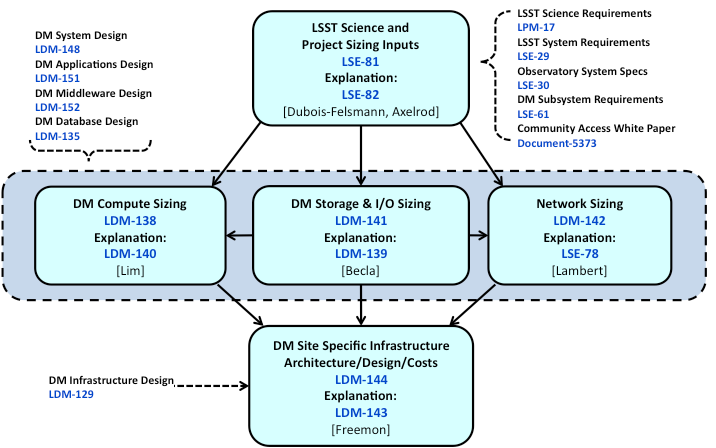
\includegraphics[width=\textwidth]{SizingModel.png}
\caption{DMS Infrastructure Sizing and Estimation}
\label{fig:sizing-model}
\end{figure}

Key input parameters include camera characteristics, the expected cadence of
observations, the number of observed stars and galaxies expected per band, the
processing operations per data element, the data transfer rates between and
within processing locations, the ingest and query rates of input and output
data, the alert generation rates, and latency and throughput requirements for
all data products. 

Processing requirements were extrapolated from the functional model of
operations, prototype pipelines and algorithms, and existing precursor
pipelines adjusted to LSST scale.  As a part of every Data Release, all data
previously processed are reprocessed with the latest algorithms, calibration
products, and parameters. This causes the processing requirements to increase
with time.  Advances in hardware performance, however, are expected to reduce
the number of nodes needed and the power and cooling devoted to them. This causes some of the performance figures in Table \ref{table:compute-sizing} to reach
a high-water mark during the survey.

\begin{table}
\centering
\begin{longtable}{|c|c|c|c|}
\hline
	& & \textit{Archive Site} & \textit{Base Site} \\ \hline
\multirow{4}{*}{Compute} & TeraFLOPS (sustained) & 197 $\rightarrow$ 970 & 30 $\rightarrow$ 62 \\ \cline{2-4}
  & Nodes & 436 $\rightarrow$ 305 (455 hwm) & 56 $\rightarrow$ 17 (59 hwm) \\ \cline{2-4}
  & Cores & 18K $\rightarrow$ 62K & 3K $\rightarrow$ 4K \\ \hline
\multirow{2}{*}{Database} & TeraFLOPS (sustained) & 40 $\rightarrow$ 310 & 55 $\rightarrow$ 306 \\ \cline{2-4}
  & Nodes & 94 $\rightarrow$ 113 (148 hwm) & 108 $\rightarrow$ 98 (133 hwm) \\ \cline{2-4}
\multirow{3}{*}{Facilities} & Floor Space & 826 $\rightarrow$ 744 ft$^2$ (834 hwm) & 278 $\rightarrow$ 195 ft$^2$ (435 hwm) \\ \cline{2-4}
  & Power & 274 $\rightarrow$ 273 kW (309 hwm) & 158 $\rightarrow$ 248 kW (248 hwm) \\ \cline{2-4}
  & Cooling & 0.9 $\rightarrow$ 0.9 mmbtu (1.1 hwm) & 0.5 $\rightarrow$ 0.8 mmbtu (0.8 hwm) \\ \hline
\end{longtable}
\caption{DMS Compute Infrastructure Sizing; growth from Survey Year 1 to Year 10; hwm = high-water mark}
\label{table:compute-sizing}
\end{table}

Storage and input/output requirements were extrapolated from the data model of
LSST data products, the DMS and precursor database schemas, and
existing database management system overhead factors in precursor
surveys and experiments adjusted to LSST scale. A summary of key numbers is
in Table \ref{table:storage-sizing}.

\begin{table}
\centering
\begin{longtable}{|c|c|c|c|}
\hline
	& & \textit{Archive Site} & \textit{Base Site} \\ \hline
\multirow{3}{*}{File Storage} & Capacity & 24 $\rightarrow$ 81 PB & \\ \cline{2-4}
  & Drives & 1602 $\rightarrow$ 862 & 597 $\righarrow$ 249 \\ \cline{2-4}
  & Bandwidth & 493 $\rightarrow$ 714 GB/s (752 hwm) & 223 $\rightarrow$ 231 GB/s (236 hwm) \\ \hline
\multirow{3}{*}{Database} & Capacity & 29 $\rightarrow$ 99 PB & 16 $\rightarrow$ 72 PB \\ \cline{2-4}
  & Drives & 3921 $\rightarrow$ 2288 & 2190 $\rightarrow$ 1642 \\ \cline{2-4}
  & Bandwidth & 1484 $\rightarrow$ 2040 GB/s (2163 hwm) & 829 $\rightarrow$ 1169 GB/s (1615 hwm) \\ \hline
\multirow{3}{*}{Tape Storage} & Capacity & 31 $\rightarrow$ 242 PB & \\ \cline{2-4}
  & Tapes & 2413 $rightarrow$ 3691 (4117 hwm) & \\ \cline{2-4}
  & Tape Bandwidth & 36 $rightarrow$ 65 GB/s & \\ \hline
\end{longtable}
\caption{DMS Storage Infrastructure Sizing; growth from Survey Year 1 to Year 10}
\label{table:storage-sizing}
\end{table}

Communications requirements were developed and modeled for the data transfers
and user query/response load, extrapolated from existing surveys and adjusted
to LSST scale.  These requirements are illustrated in Figures \ref{fig:near-real-time-flows} for per-visit transfers and Figure \ref{fig:annual-reprocessing-flows} for annual transfers.  Peak bandwidths assume 5 seconds for international
image transfer and 30 days to transfer Data Release catalogs from NCSA to the
Chilean DAC.

\begin{figure}
\centering
\includegraphics[width=\textwidth]{NearRealTimeDataFlow.pdf}
\caption{Near Real-Time Data Flows}
\label{fig:near-real-time-flows}
\end{figure}

\begin{figure}
\centering
\includegraphics[width=\textwidth]{AnnualReprocessingDataFlow.pdf}
\caption{Annual Reprocessing Data Flows}
\label{fig:annual-reprocessing-flows}
\end{figure}

In all of the above, industry-provided technology trends (\citeds{LDM-143})
were used to extrapolate to the LSST construction and operations phases in
which the technology will be acquired, configured, deployed, operated, and
maintained. A just-in-time acquisition strategy is employed to leverage
favorable cost/performance trends. 

The resulting performance and sizing requirements show the DMS to be a
supercomputing­-class system with correspondingly large data input/output and
network bandwidth rates.  Despite this size, technology trends show this to be
well within the anticipated performance of commodity-based systems during the
construction and operations time frame.



\section{Component Overview}\label{component-overview}

The services that make up the DMS are in turn made up of software and
underlying service components, instantiated in a particular
configuration in a particular computing environment to perform a
particular function. Some software components are specific to a service;
others are general-purpose and reused across multiple services. Many
services have only one instance in the production system; others have
several, and all have additional instances in the development and
integration environments for testing purposes.

The DMS services can be considered to consist of four tiers of software
components. The top tier is the LSST Science Platform, which is deployed
in the DACs and other computational environments to provide a user
interface and analysis environment for science users and LSST staff. The
detailed design of this tier is given in ``LSST Science Platform,'' \citeds{LDM-542}. The next
tier is composed of science ``applications'' software that generates
data products. This software is used to build ``payloads'', sequences of
pipelines, that perform particular data analysis and product generation
tasks. It is also used by science users and staff to analyze the data
products. The detailed design of the components in this tier is given in
Data Management Science Pipelines Design, \citeds{LDM-151}. A lower tier is
``middleware'' software components and services that execute the science
application payloads and isolate them from their environment, including
changes to underlying technologies. These components also provide data
access for science users and staff. The detailed design of the
components in this tier is given in Data Management Middleware Design,
\citeds{LDM-152}. The bottom tier is ``infrastructure'': hardware, networking,
and low-level software and services that provide a computing
environment. The detailed design of components in this tier is given in
Data Management Services \& Infrastructure, \citeds{LDM-129}, and Network Design,
\citeds{LSE-78}.

The DMS computing environments reside in four main physical locations:
the Summit Site including the main Observatory and Auxiliary Telescope
buildings on Cerro Pachon, Chile; the Base Facility data center located
at the Base Site in La Serena, Chile; the Archive Facility data center
at the National Center for Supercomputing Applications (NCSA) in Urbana,
Illinois, USA; and the Satellite Computing Facility at CC-IN2P3 in Lyon,
France. These are linked by high-speed networks to allow rapid data
movement. The Base and Archive Facilities include production
computational environments (the Base Enclave and NCSA Enclave,
respectively) and also the US and Chilean Data Access Centers. In
addition, a Commissioning Cluster computational environment also resides
at the Base Facility.

The DMS service instances in the NCSA Enclave can be broken down into
three main functional domains: a near-realtime online domain (L1)
closely linked to the rest of the Observatory; an offline Level 2 domain
(L2) organized primarily around the annual Data Release Production; and
an analysis and developer support domain (ADS) encompassing environments
that operations staff use for science validation, software development,
system integration, and system testing. In addition, an underlying
infrastructure domain (Infra) hosts services supporting all of the other
domains, including a common Data Backbone that provides data transport
and archiving and that is the primary connection between all of the
domains. These domains are distinguished by having different users,
operations timescales, interfaces, and often components.

The service instances that make up the DMS include (with the
computational environment or domains they are in noted):
\begin{itemize}
\item
  Image and EFD Archiving (Base)
\item
  Prompt Processing Ingest (Base)
\item
  Observatory Control System (OCS) Driven Batch Control (Base)
\item
  Telemetry Gateway (Base)
\item
  Prompt Processing (L1)
\item
  OCS Driven Batch Processing (L1)
\item
  Offline Processing (L1)
\item
  Alert Distribution (L1)
\item
  Alert Filtering (L1)
\item
  Level 1 Quality Control (QC) (L1)
\item
  Template and Calibration Products Production Execution (L2)
\item
  Data Release Production Execution (L2)
\item
  Data Release Production Satellite Processing (Satellite Computing)
\item
  Level 2 QC (L2)
\item
  LSST Science Platform Commissioning Cluster instance (Commissioning
  Cluster)
\item
  LSST Science Platform Data Access Center instances (DACs)
\item
  Bulk Data Distribution (DAC)
\item
  LSST Science Platform Science Validation instance (ADS)
\item
  Developer Services (ADS)
\item
  Integration and Test (ADS)
\item
  Data Backbone (Infra)
\item
  Management/Monitoring (Infra)
\item
  Provisioning/Deployment (Infra)
\item
  Workload/Workflow (Infra)
\item
  HTCondor Batch Processing (Infra)
\item
  Identity Management (Infra)
\end{itemize}

The relationships between these services, their deployment environments,
functional domains, and science application ``payloads'' can be
visualized in Figure~\ref{fig:deployment}.

\begin{figure}
\centering
\includegraphics[height=0.9\textheight]{images/DMSDeployment.pdf}
\caption{Data Management System Deployment}
\label{fig:deployment}
\end{figure}

The common infrastructure services are illustrated in Figure~\ref{fig:commonservices}.

\begin{figure}
\centering
\includegraphics[height=0.9\textheight]{images/DMSCommonServices.pdf}
\caption{Data Management System Common Infrastructure Services}
\label{fig:commonservices}
\end{figure}

The science application software for the Alert Production, daytime
processing, Data Release Production, and calibration processing is built
out of a set of frameworks that accept plugins. In turn, those
frameworks build on middleware that provides portability and
scalability.  The relationships between the packages implementing
these se frameworks and plugins and the underlying middleware packages
are shown in Figure~\ref{fig:scipi}.

Key applications software components include:
\begin{itemize}
\item
  Low-level astronomical software primitives and data structures
  (\texttt{afw})
\item
  Image processing and measurement framework with core algorithms
  (\texttt{ip\_*}, \texttt{meas\_*})
\item
  Additional image processing and measurement algorithms
  (\texttt{meas\_extensions\_*})
\item
  High-level algorithms and driver scripts that define pipelines
  (\texttt{pipe\_tasks}, \texttt{pipe\_drivers})
\item
  Camera-specific customizations (\texttt{obs\_*})
\end{itemize}

\begin{figure}
\centering
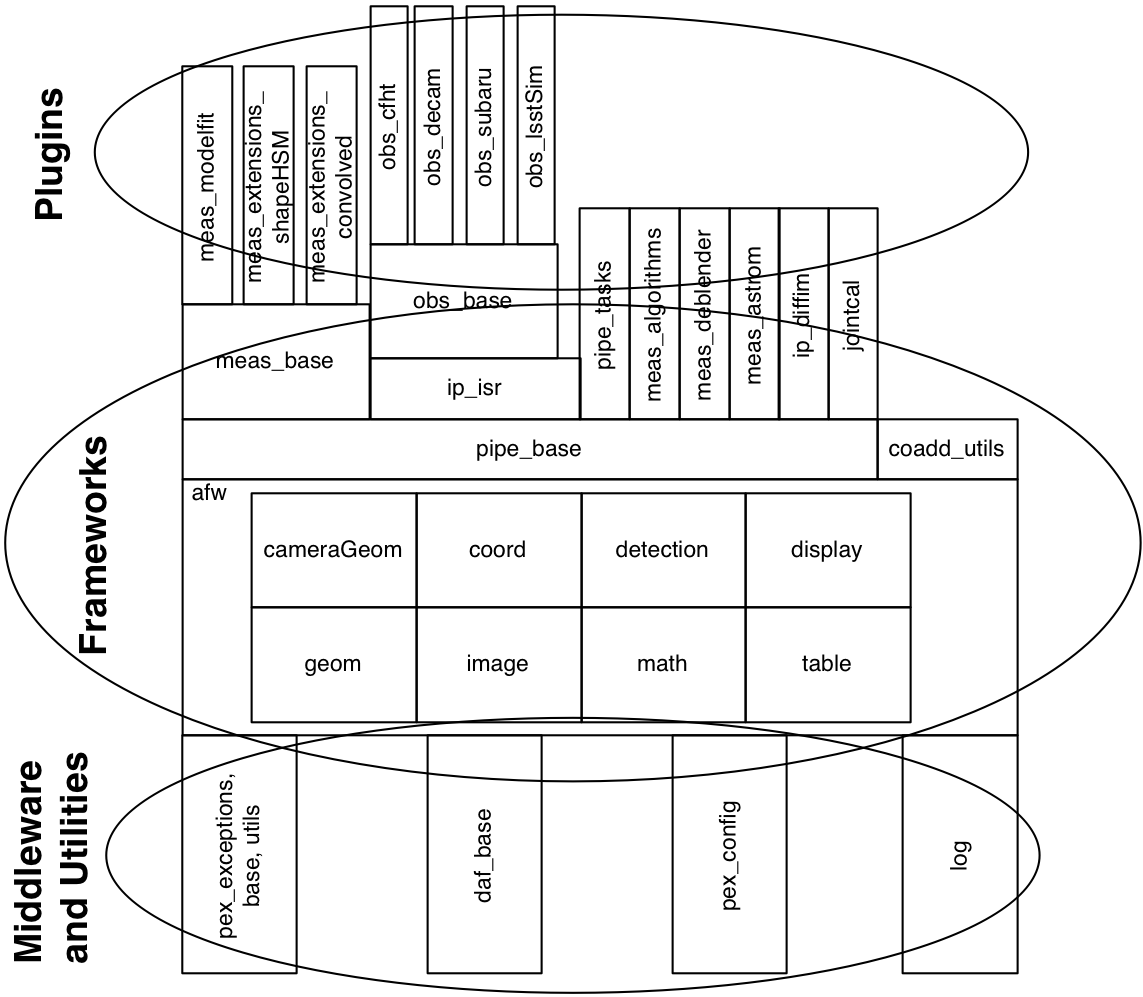
\includegraphics[width=\textwidth]{images/DM_Application_Software_Arch.png}
\caption{Data Management Science Pipelines Software ``Stack''}
\label{fig:scipi}
\end{figure}

Key middleware components include:
\begin{itemize}
\item
  Data access client (Data Butler) (\texttt{daf\_persistence})
\item
  Parallel distributed database (\texttt{qserv})
\item
  Task framework (\texttt{pex\_*}, \texttt{log}, \texttt{pipe\_base},
  \texttt{ctrl\_pool})
\item
  Workflow and orchestration for production control (\texttt{ctrl\_*})
\end{itemize}

Infrastructure components include:
\begin{itemize}
\item
  Other databases (typically relational)
\item
  Filesystems
\item
  Authentication and authorization (identity management)
\item
  Provisioning and resource management
\item
  Monitoring
\end{itemize}

The relationships between the middleware and infrastructure components
are illustrated in Figure~\ref{fig:mwandinfra}.

\begin{figure}
\centering
\includegraphics[width=\textwidth]{images/MiddlewareInfrastructure.pdf}
\caption{Data Management Middleware and Infrastructure}
\label{fig:mwandinfra}
\end{figure}

\section{Base Enclave}\label{base-enclave}

Services located in this enclave are located at the Base solely because
they must interact with the OCS or the Camera Data System (also known as
the Camera DAQ) or both. In several cases, services located here
interact closely with corresponding services in the NCSA Enclave's Level
1 Domain, to the point where the Base service cannot function if the
NCSA service is not operational. This reliance has been taken into
account in the fault tolerance strategies used.

The primary goals of the services in this enclave are to transfer data
to appropriate locations, either to NCSA, from NCSA, or to the Data
Backbone.

The services in this enclave and their partners in the NCSA Enclave
Level 1 Domain need to run rapidly and reliably. They run at times
(outside office hours) and with latencies that are not amenable to a
human-in-the-loop design. Instead, they are designed to execute
autonomously, often under the control of the OCS, with human oversight,
monitoring, and control only at the highest level.

\subsection{Service Descriptions}\label{base-service-descriptions}

Detailed concepts of operations for each service can be found in
``Concept of Operations for the LSST Production Services'' (\citeds{LDM-230}).


\subsubsection{Image and EFD Archiving}\label{image-and-efd-archiving}

This component is composed of several Image Archiving service and
Catch-Up Image Archiving instances: one pair each for the LSSTCam, the
ComCam, and the Auxiliary Telescope Spectrograph, all of which may be
operated simultaneously. These capture raw images taken by each camera,
including the wavefront sensors and the guide sensors of the LSSTCam or
ComCam when so configured, retrieving them from their respective Camera
Data System instances. They also capture specific sets of metadata
associated with the images, including telemetry values and event
timings, from the OCS publish/subscribe middleware and/or from the EFD.
The image pixels and metadata are then permanently archived in the Data
Backbone. The catch-up versions archive into the Data Backbone any raw
images and metadata that were missed by the primary archiving services
due to network or other outage, retrieving them from the flash storage
in the Camera Data System instances and the EFD.

This component also includes an EFD Transformation service that extracts
all information (including telemetry, events, configurations, and
commands) from the EFD and its large file annex, transforms it into a
form more suitable for querying by image timestamp, and loads it into
the permanently archived ``Transformed EFD'' database in the Data
Backbone.

\subsubsection{Prompt Processing Ingest}\label{prompt-processing-ingest}

This component is composed of two instances that capture
crosstalk-corrected images from the LSSTCam and ComCam Camera Data
Systems along with selected metadata from the OCS and/or EFD and
transfer them to the Prompt Processing service in the NCSA Enclave Level
1 Domain.

There is no Prompt Processing Ingest instance for the auxiliary
telescope spectrograph.

\subsubsection{OCS Driven Batch Control}\label{ocs-driven-batch-control}

This service receives commands from the OCS and invokes the OCS Driven
Batch Processing service in the NCSA Enclave Level 1 Domain to execute
corresponding science payloads. It is used for modest-latency analysis
of images during Commissioning and for processing daily calibration
images in normal observing operations. A summary status for the
processing performed is returned to the OCS for each command, following
the normal OCS commanding protocol.

\subsubsection{Telemetry Gateway}\label{telemetry-gateway}

This service obtains information from the NCSA Enclave Level 1 Domain,
particularly status and quality metrics from Prompt Processing of images
and the Level 1 Quality Control service, and transmits it to the OCS as
specified in the Data Management-OCS Software Communication Interface
(\citeds{LSE-72}). Note that more detailed information on the status and
performance of DMS services will also be available to Observatory
operators through remote displays originated from the
Management/Monitoring infrastructure services in all DMS computational
environments.

\subsection{Interfaces}\label{base-interfaces}

OCS to all Base Enclave services: these interface through the SAL
library provided by the OCS subsystem.

Archiver and Catch-Up Archiver to Data Backbone: files are copied to
Data Backbone storage via a file transfer mechanism, and their
information and metadata are registered with Data Backbone management
dataabases. The Data Butler is not used for this low-level,
non-science-payload interface.

EFD to EFD Transformer: this interface is via connection to the
databases that make up the EFD as well as file transfer from the EFD's
Large File Annex.

EFD Transformer to Data Backbone: Transformed EFD entries are inserted
into the ``Transformed EFD'' database resident within the Data Backbone.

Camera Data System to Archiver, Catch-Up Archiver, Prompt Processing
Ingest: these interface through the custom library provided by the
Camera Data System.

Prompt Processing Ingest to Prompt Processing: BBFTP is used to transfer
files over the international network from the ingest service to the
processing service.

OCS Driven Batch Control to OCS Driven Batch Processing: HTCondor is
used to transfer execution instructions over the international network
from the control service to the processing service and return status and
result information.

Telemetry Gateway from NCSA Enclave Level 1 Domain services: RabbitMQ is
used to transfer status and quality metrics to the gateway over the
international network.

\section{NCSA Enclave Level 1 Domain}\label{ncsa-enclave-level-1-domain}

This domain is responsible for the compute-intensive processing for all
near-realtime operations and other operations closely tied with the
Observatory. Its primary goals are to process images and metadata from
the Observatory into ``online'' science data products and publish them
to the DACs, alert subscribers, and back to the OCS.

The Prompt Processing, OCS Driven Batch Processing, and Offline
Processing services support execution of science payloads in three
different ways. Prompt Processing is tightly integrated with the
observing cadence and is intended to function in near-realtime with
strict result deadlines. OCS Driven Batch Processing is invoked by the
OCS but has more modest latency requirements. Offline Processing is not
invoked by the OCS but operates under DMS control, typically during the
daytime.

The Alert Distribution and Alert Filtering services receive batches of
alerts resulting from Prompt Processing of each scienc visit; they then
provide alert streams to community alert brokers and LSST data rights
holders, respectively.

The Level 1 Quality Control service monitors the ``online'' science data
products, including alerts, notifying operators if any anomalies are
found.

Like the services in the Base Enclave, these services need to run
rapidly and reliably and so are designed to execute autonomously.

\subsection{Service Descriptions}\label{ncsa-l1-service-descriptions}

Detailed concepts of operations for each service can be found in
``Concept of Operations for the LSST Production Services'' (\citeds{LDM-230}).

\subsubsection{Prompt Processing}\label{prompt-processing}

This service receives crosstalk-corrected images and metadata from the
Prompt Processing Ingest service at the Base and executes the Alert
Production science payload on them, generating ``online'' data products
that are stored in the Data Backbone. The Alert Production payload then
sends alerts to the Alert Distribution service.

The Prompt Processing service has calibration (including Collimated Beam
Projector images), science, and deep drilling modes. In calibration
mode, it executes a Raw Calibration Validation payload that provides
rapid feedback of raw calibration image quality. In normal science mode,
two consecutive exposures are grouped and processed as a single visit.
Definitions of exposure groupings to be processed as visits in deep
drilling and other modes are TBD. The service is required to deliver
Alerts within 60 seconds of the final camera readout of a standard
science visit with 98\% reliability.

There is no Prompt Processing service instance for the Auxiliary
Telescope Spectrograph.

\subsubsection{OCS Driven Batch
Processing}\label{ocs-driven-batch-processing}

This service executes science payloads in response to commands from the
OCS Driven Batch Control service at the Base and thus indirectly from
the Observatory Control System. It is used for modest-latency analysis
of images during Commissioning and for processing daily calibration
images in normal observing operations. Images and metadata are taken
from the Data Backbone, and results are provided back to the Data
Backbone; there is no direct connection from this service to the Camera
Data System. This obviously bounds the minimum latency from image
acquisition to processing start by the latency of the Archiving service
and Data Backbone transfer. A summary status for the processing
performed is sent to the OCS Driven Batch Control service to be returned
to the OCS.

\subsubsection{Offline Processing}\label{offline-processing}

This service executes science payloads to ensure that all Level 1 data
products are generated within 24 hours. In particular, this service
executes the daytime Moving Object Processing System payload. It also
may execute a variant of the Alert Production payload if the Prompt
Processing service encounters difficulties. Images and metadata are
taken from the Data Backbone, and results are provided back to the Data
Backbone.

\subsubsection{Level 1 Quality Control}\label{level-1-quality-control}

This service collects information on Level 1 science and calibration
payload execution, post-processes the science data products from the
Data Backbone to generate additional measurements, and monitors the
measurement values against defined thresholds, providing an automated
quality control capability for potentially detecting issues with the
environment, telescope, camera, data acquisition, or data processing.
Alarms stemming from threshold crossings are delivered to Observatory
operators and to LSST Data Facility Production Scientists for
verification, analysis, and resolution.

\subsubsection{Alert Distribution}\label{alert-distribution}

This service obtains alerts generated by the Alert Production science
payload and distributes them to community alert brokers and to the Alert
Filtering service.

\subsubsection{Alert Filtering}\label{alert-filtering}

This service obtains an alert feed from the Alert Broker Feed service
and allows individual LSST data rights holders to execute limited
filters against it, producing filtered feeds that are then distributed
to the individuals.

\subsection{Interfaces}\label{ncsa-l1-interfaces}

Prompt Processing to Alert Distribution and Alert Filtering: these
interface through a reliable transport system.

Prompt Processing to Offline Processing: in the event that Prompt
Processing runs over its allotted time window, processing can be
cancelled and the failure recorded, after which Offline Processing will
redo the processing at a later time. Note that it may be possible, if
sufficient computational resources have been provisioned, for the Prompt
Processing to be allowed to continue to run, with spare capacity used to
maintain latency for future visits. In that case, there would
effectively be an infinite time window.

Science Payloads to Data Backbone: payloads use the Data Butler as a
client to access files and catalog databases within the Data Backbone.

\section{NCSA Enclave Level 2 Domain}\label{ncsa-enclave-level-2-domain}

This domain is responsible for all longer-period data processing
operations, including the largest and most complex payloads supported by
the DMS: the annual Data Release Production (DRP) and periodic
Calibration Products Productions (CPPs). Note that CPPs will execute
even while the annual DRP is executing, hence the need for a separate
service. The Level 2 Quality Control Service monitors the science data
products, notifying operators if any anomalies are found.

The services in this domain need to run efficiently and reliably over
long periods of time, spanning weeks or months. They need to execute
millions or billions of tasks when their input data becomes available
while tracking the status of each and preserving its output. They are
designed to execute autonomously with human oversight, monitoring, and
control primarily at the highest level, although provisions are made for
manual intervention if absolutely necessary.

This domain does not have direct users (besides the operators of its
services); the services within it obtain inputs from the Data Backbone
and place their outputs into the Data Backbone.

\subsection{Service Descriptions}\label{ncsa-l2-service-descriptions}

\subsubsection{Template and Calibration Products Production
Execution}\label{template-and-calibration-products-production-execution}

This service executes various CPP science payloads at intervals to
generate Master Calibration Images and populate the Calibration Database
with information derived from analysis of raw calibration images from
the Data Backbone and information in the Transformed EFD. This includes
the computation of crosstalk correction matrices. Although not a
calibration product, the templates used by Alert Production are also
generated by this service, based on raw science images from the Data
Backbone. Additional information such as external catalogs are also
taken from the Data Backbone. The intervals at which this service
executes will depend on the stability of Observatory systems but are
expected to include at least monthly and annual executions. The annual
execution is a prerequisite for the subsequent execution of the Data
Release Production. The service involves human scientist/operator input
to determine initial configurations of the payload, to monitor and
analyze the results, and possibly to provide additional configuration
information during execution.

\subsubsection{Data Release Production
Execution}\label{data-release-production-execution}

This service executes the DRP science payload annually to generate all
Level 2 data products after the annual CPP is executed. A small-scale
(about 10\% of the sky) mini-production is executed first to ensure
readiness, followed by the full production. Raw science images are taken
from the Data Backbone along with Master Calibration Images and
information from the Transformed EFD. Additional information such as
external catalogs may also be taken from the Data Backbone. Computing is
performed in conjunction with the DRP Satellite Processing service at
CC-IN2P3, which will have capacity for half of the DRP processing.
Output data products from both the mini-production and the main
production are loaded into the Data Backbone, including both images and
catalogs. From there, they are analyzed by LSST staff scientists and
selected external scientists using the Science Validation instance of
the LSST Science Platform to ensure quality and readiness for release.
The to-be-released data products are loaded into the Data Access Center
services, and access is then enabled on the release date. The service
involves human scientist/operator/programmer input to determine initial
configurations of the payload, to monitor and analyze results, and, when
absolutely necessary, to make ``hot fixes'' during execution that
maintain adequate consistency of the resulting data products.

\subsubsection{Level 2 Quality Control}\label{level-2-quality-control}

This collects information on Level 2 science payload execution,
post-processes the science data products from the Data Backbone to
generate additional measurements, and monitors the measurement values
against defined thresholds, providing an automated quality control
capability for potentially detecting issues with the data processing but
also the environment, telescope, camera, or data acquisition. Alarms
stemming from threshold crossings are delivered to LSST Data Facility
Production Scientists for verification, analysis, and resolution.

\subsection{Interfaces}\label{ncsa-l2-interfaces}

Calibration Products Production Execution and Data Release Production
Execution to Data Backbone: for large-scale productions, a workflow
system is expected to stage files and selected database entries from the
Data Backbone to local storage for access by the science payloads via
the Data Butler. Similarly, the staging system will ingest output images
and catalogs into the Data Backbone.

\section{Satellite Computing Enclave}\label{satellite-computing-enclave}

\subsection{Service Description}\label{satellite-service-description}

\subsubsection{Data Release Production Satellite
Processing}\label{data-release-production-satellite-processing}

This service controls the processing of jobs on the CC-IN2P3 satellite
computing facilities under the overall workload and workflow management
of the Data Release Production Execution service at NCSA.

\subsection{Interfaces}\label{satellite-interfaces}
DRP Satellite Processing to DRP Execution: DRP Execution will stage data
to the Satellite Processing facility.  All raw data, including images,
metadata, and the Transformed EFD, will be transferred.  Intermediate
data products will be transferred back to the NCSA Enclave Level 2 Domain.


\section{Data Access Center Enclaves}\label{data-access-center-enclaves}

There are two Data Access Centers, one in the US at NCSA and one in
Chile at the Base. These DACs are responsible for all
science-user-facing services, primarily instances of the LSST Science
Platform (LSP). The LSP is the preferred analytic interface to LSST data
products in the DAC. It provides computation and data access on both
interactive and asynchronous timescales. The US DAC also includes a
service for distributing bulk data on daily and annual (Data Release)
timescales to partner institutions, collaborations, and LSST Education
and Public Outreach (EPO).

The services in this domain must support multiple users simultaneously
and securely. The LSP must be responsive to science user needs; updates
are likely to occur at a different cadence from the other domains as a
result. The LSP must operate reliably enough that scientific work is not
impeded.

\subsection{Service Descriptions}\label{dac-service-descriptions}

\subsubsection{Bulk Data Distribution}\label{bulk-data-distribution}

This service is used to transmit Level 1 and Level 2 data products to
partners such as LSST Education and Public Outreach, the UK LSST
project, and the Dark Energy Science Collaboration. It extracts data
products from the Data Backbone and transmits them over high bandwidth
connections to designated, pre-subscribed partners.

\subsubsection{LSST Science Platform DAC
instances}\label{lsst-science-platform-dac-instances}

This service provides an exploratory analysis environment for science
users. It can be further broken down into three ``Aspects'' that it
presents to end users, along with underlying ``backend services'' that
users can take advantage of, as illustrated in Figure~\ref{fig:lsp}.

\begin{figure}
\centering
\includegraphics[width=0.5\textwidth]{images/SciencePlatform.pdf}
\caption{LSST Science Platform}
\label{fig:lsp}
\end{figure}

The ``Portal'' Aspect provides a pre-specified yet flexible discovery,
query, and viewing tool. The ``JupyterLab'' Aspect provides a fully
flexible (``notebook'') environment incorporating rendering of images,
catalogs, and plots and providing for execution of LSST-provided and
custom algorithms. The ``Web API'' Aspect provides a
language-independent, VO-compliant Web Services data access API with
extensions for LSST capabilities and volumes. Access is provided via all
three Aspects to all data products, including images, catalogs, and
metadata. The Web API Aspect regenerates ``virtual'' data products on
demand when required.

The backend services provide general-purpose user computation, including
batch job submission; user file storage accessible to all three Aspects;
and user database storage for relational tables.  Data may be shared with
individual users, with groups, or with all DAC users (data rights
holders). Resource management of the backend services is based on a
small ``birthright'' quota with additional resources allocated by a
committee.

All usage of any LSST Science Platform instance requires authentication
to ensure availability only to LSST data rights holders or LSST
operations staff.

\subsection{Interfaces}\label{dac-interfaces}

Bulk Data Distribution and LSST Science Platform to Data Backbone: Both
DAC-resident services retrieve their data, including raw images, nightly and
annual image and catalog data products, metadata, and provenance, from the Data
Backbone.  The LSP Portal Aspect uses the LSP Web APIs to retrieve data.  The
LSP JupyterLab Aspect can use the LSP Web APIs and also can use the Data Butler
client library to access the Data Backbone.

Bulk Data Distribution to partners: The exact delivery mechanism for
large-scale data distribution is TBD.


\section{NCSA Enclave Analysis and Developer Support
Domain}\label{ncsa-enclave-analysis-and-developer-support-domain}

This domain encompasses environments for analysts, developers, and
integration and test. Its users are the Observatory staff as they
analyze raw data and processed data products to characterize them,
develop new algorithms and systems, and test new versions of components
and services before deployment.

\subsection{Service Descriptions}\label{ncsa-ads-service-descriptions}

\subsubsection{LSST Science Platform Science Validation
instance}\label{lsst-science-platform-science-validation-instance}

This instance of the LSST Science Platform is customized to allow access
to unreleased and intermediate data products from the Alert, Calibration
Products, and Data Release Productions. It is optimized for usage by
scientists within the LSST Operations team, although selected external
scientists can be granted access to assist with Science Validation. Part
of the optimization is to size and configure the three Aspects of the
LSP appropriately; in particular, more JupyterLab usage and less portal
usage is expected.

\subsubsection{Developer Services}\label{developer-services}

Software version control service, packaging, build and unit test
service, software release management, ticket tracking service,
documentation services, etc.

\subsubsection{Integration and Testing}\label{integration-and-testing}

Integration environments representing various deployment environments,
deployment services, test datasets, test execution services, metric measurement
and tracking services, etc.  This service includes the DM instance of the
Camera DAQ Test Stand, used in a Base Enclave integration environment, as well
as the Prototype Data Access Center (PDAC), which is a Data Access Center
Enclave integration environment.

\subsection{Interfaces}\label{ncsa-ads-interfaces}

LSP Science Validation instance and Integration and Testing to Data Backbone:
All three services in this domain interface with the Data Backbone.  The LSP
Science Validation instance is used to inspect, analyze, and validate the data
products of the Data Release Production prior to their release and so has
access to those products in the Data Backbone; since it may be used to annotate
the data products, it can also write to the Data Backbone.  The Integration and
Testing environment may use raw data, intermediate data products, and final
data products to perform tests.

Developer Services do not have direct interfaces with the rest of the
operational system; they communicate via the distributed source version control
system, the package management system, and the configuration system.  There is
a separate Developer Services instance of the Data Backbone to manage and track
datasets used during development.


\section{Commissioning Cluster}\label{commissioning-cluster}

\subsection{Service Description}\label{commcluster-service}

\subsubsection{LSST Science Platform Commissioning
instance}\label{lsst-science-platform-commissioning-instance}

This instance of the LSST Science Platform for Science Validation runs
on the Commissioning Cluster at the Base Facility (but also has access
to computational resources at the Archive) and accesses a Base endpoint
for the Data Backbone. This location at the Base lowers the latency of
both access to Data Backbone-resident data (which does not have to wait
for transfer over the international network) and, perhaps more
importantly, for user interface operations for staff in Chile, which are
served locally. Note that the Commissioning Cluster does not have direct
access to the Camera Data System; it relies on the Archiver service to
obtain data. The Commissioning Cluster will have direct access to the
OCS's Base replica of the EFD (before transformation).

\subsection{Interfaces}\label{commcluster-interfaces}

Commissioning Cluster to Data Backbone: The Commissioning Cluster relies on the
Data Backbone for its data, like the other instances of the LSST Science
Platform.

Commissioning Cluster to EFD: The Commissioning Cluster has direct read-only
client access to the Base replica of the EFD (before transformation).


\section{Infrastructure Domain}\label{infrastructure-domain}

This domain encompasses the underlying services and systems that form
the computing environments in which the other domains are deployed and
operate. It interfaces with the other domains but has no direct users.

\subsection{Service Descriptions}\label{infrastructure-service-descriptions}

\subsubsection{Data Backbone}\label{data-backbone}

The Data Backbone is a key component that provides for data storage,
transport, and replication, allowing data products to move between
computational environments. This service provides policy-based
replication of files (in the Science Image Archive) and databases (in
the Science Catalog Archive) across multiple physical locations,
including the Base, Commissioning Cluster, NCSA, and DACs. It manages
caches of files at each endpoint as well as persistence to long-term
archival storage (e.g. tape). It provides a registration mechanism for
new datasets and database entries and a retrieval mechanism compatible
with the Data Butler.

The Qserv distributed database system for large-scale catalog data has
instances within the Data Backbone in each DAC as well as in the NCSA
Enclave.

The relationships between the Data Backbone components are illustrated
in Figure~\ref{fig:dbb}.

\begin{figure}
\centering
\includegraphics[width=0.7\textwidth]{images/DataBackbone.pdf}
\caption{Data Backbone}
\label{fig:dbb}
\end{figure}

\subsubsection{Management/Monitoring}\label{managementmonitoring}

These services provide management and monitoring at service and
infrastructure systems levels for each enclave and domain.

\subsubsection{Provisioning/Deployment}\label{provisioningdeployment}

These services provide compute, local-to-node storage, and local-to-LAN
storage resources for all processing, including Prompt Processing, Batch
Processing, and the Science Platforms. They allow allocation of compute
and storage resources as well as reproducible, controlled deployment of
services onto those resources.

Some compute resources are reserved for particular uses, but others can
be flexibly provisioned, up to a certain maximum quota, if needed to
deal with surges in processing.

The priority order for processing is:
\begin{itemize}
\item
  Prompt processing
\item
  Offline processing
\item
  OCS-controlled batch processing
\item
  LSP Commissioning Cluster processing
\item
  LSP Science Validation processing
\item
  LSP Data Access Center processing
\item
  Template and Calibration Products Production
\item
  Data Release Production
\end{itemize}

The Base Enclave's services are not highly dynamic or flexible, as they
primarily provide interfacing to the OCS and Camera Data System. The
baseline provisioning for them is using vSphere; they will be deployed
using Puppet.

\subsubsection{Workload/Workflow}\label{workloadworkflow}

These services provide management of the execution of science payloads
ranging from a single pipeline to a series of ``campaigns'', each
consisting of multiple pipelines. They are able to handle massively
distributed computing, executing jobs when their inputs become available
and tracking their status and outputs. They ensure that the data needed
for a job is accessible to it and that outputs (including log files, if
any) are preserved. They can allocate work across multiple computing
environments, in particular between NCSA and the Satellite Computing
Facility at CC-IN2P3.

\subsubsection{Batch Processing}\label{batch-processing}

This service provides execution of batch jobs with a variety of
priorities from a variety of users in a variety of environments (e.g. OS
and software configurations) on the underlying provisioned compute
resources. It will use containerization to handle heterogeneity of
environments. HTCondor is the baseline technology choice for this
service.

\subsubsection{Identity Management}\label{identity-management}

This service provides authentication and authorization for all users of
any DMS component, especially the LSST Science Platform instances.

\subsection{Interfaces}\label{infrastructure-interfaces}

The infrastructure services generally interact with all other deployed
services.  In the Base Enclave, there is no workload/workflow management or
batch processing; provisioning and deployment are also simplified.

Identity management instances are present in the Base and NCSA Enclaves.
(Another replica will be maintained at the Summit.)  These are used to support
authentication and authorization for the other physically co-located enclaves:
the Commissioning Cluster and the two Data Access Centers.


\section{Software Components}\label{software-components}

\subsection{Science Payloads}\label{science-payloads}

These payloads are described in more detail in the DM Applications Design
Document (\citeds{LDM-151}). Payloads are built from application software
components.

\subsubsection{Alert Production Payload}\label{alert-production-payload}

Executes under control of the Prompt Processing service. Generates all
Level 1 science data products including Alerts (with the exception of
Solar System object orbits) and loads them into the Data Backbone and
Level 1 Database. Transmits Alerts to Alert Distribution service.
Generates image quality feedback to the OCS and observers via the
Telemetry Gateway. Uses crosstalk-corrected science images and
associated metadata delivered by the Prompt Processing service; uses
Master Calibration Images, Template Images, Level 1 Database, and
Calibration Database information from the Data Backbone.

\subsubsection{MOPS Payload}\label{mops-payload}

Executes under control of the Offline Processing service after a night's
observations are complete. Generates entries in the MOPS Database and
the Level 1 Database, including Solar System Object records,
measurements, and orbits. Performs precovery forced photometry of
transients. Uses Level 1 Database entries and images from the Data
Backbone.

\subsubsection{Raw Calibration Validation
Payload}\label{raw-calibration-validation-payload}

Executes under control of the Prompt Processing service. Generates raw
calibration image quality feedback to the OCS and observers via the
Telemetry Gateway. Uses crosstalk-corrected science images and
associated metadata delivered by the Prompt Processing service, Master
Calibration Images, and Calibration Database information from the Data
Backbone.

\subsubsection{Daily Calibration Products Update
Payload}\label{daily-calibration-products-update-payload}

Executes under control of the OCS-controlled batch processing service so
that its execution can be synchronized with the observing schedule. Uses
raw calibration images and information from the Transformed EFD to
generate a subset of Master Calibration Images and Calibration Database
entries in the Data Backbone.

\subsubsection{Periodic Calibration Products Production
Payload}\label{periodic-calibration-products-production-payload}

Executes under control of the Template and CPP Execution service at
nominally monthly intervals but perhaps as frequently as weekly or as
infrequently as quarterly, depending on the stability of Observatory
systems and their calibrations. Uses raw calibration images and
information from the Transformed EFD to generate a subset of Master
Calibration Images and Calibration Database entries in the Data
Backbone.

\subsubsection{Template Generation
Payload}\label{template-generation-payload}

Executes under control of the Template and CPP Execution service if
necessary to generate templates for Alert Production in between annual
Data Release Productions. Uses raw science images to generate the
templates, placing them in the Data Backbone.

\subsubsection{Annual Calibration Products Production
Payload}\label{annual-calibration-products-production-payload}

Executes under control of the Template and CPP Execution service at
annual intervals prior to the start of the Data Release Production. Uses
raw calibration images, information from the Transformed EFD,
information from the Auxiliary Telescope Spectrograph, and external
catalogs to generate Master Calibration Images and Calibration Database
entries in the Data Backbone.

\subsubsection{Data Release Production
Payload}\label{data-release-production-payload}

Executes under control of the DRP Execution service at annual intervals,
first running a ``mini-DRP'' over a small portion of the sky, followed
by the full DRP over the entire sky. Produces science data products in
the Data Backbone.

\subsection{SUIT}\label{suit}

The Science User Interface and Tools provide visualization, plotting,
catalog rendering, browsing, and searching elements that can be
assembled into predetermined ``portals'' but can also be used flexibly
within dynamic ``notebook'' environments.

\subsection{Middleware}\label{middleware}

\subsubsection{Data Butler Access
Client}\label{data-butler-access-client}

The Data Butler provides an access abstraction for all science payloads
that enables their underlying data sources and destinations to be
configured at runtime with a variety of back-ends ranging from local
disk to network locations and a variety of serializations ranging from
YAML and FITS files (extensible to HDF5 or ASDF) to database tables. The
Butler client is also available within the LSST Science Platform
JupyterLab environment.

\subsubsection{Parallel Distributed Database
(Qserv)}\label{parallel-distributed-database-qserv}

Underlying the catalog data access web service is a parallel distributed
database required to handle the petabyte-scale,
tens-of-trillions-of-rows catalogs produced by LSST.

\subsubsection{Task Framework}\label{task-framework}

The Task Framework is a Python class library that provides a structure
(standardized class entry points and conventions) to organize low-level
algorithms into potentially-reusable algorithmic components (Tasks; e.g.
dark frame subtraction, object detection, object measurement), and to
organize tasks into basic pipelines (SuperTasks; e.g., process a single
visit, build a coadd, difference a visit). The algorithmic code is
written into (Super)Tasks by overriding classes and providing
implementation for standard entry points. The Task Framework allows the
pipelines to be constructed and run at the level of a single node or a
group of tightly-synchronized nodes. It allows for sub-node
parallelization: trivial parallelization of Task execution, as well as
providing (in the future) parallelization primitives for development of
multi-core Tasks and synchronized multi-node Tasks.

The Task Framework serves as an interface layer between orchestration
and the algorithmic code. It exposes a standard interface to
``activators'' (command-line runners as well as the orchestration layer
and QA systems), which use it to execute the code wrapped in tasks. The
Task Framework does not concern itself with fault-tolerant massively
parallel execution of the pipelines over multiple (thousands) of nodes
nor any staging of data that might be required; this is the concern of
the orchestration middleware.

The Task Framework exposes to the orchestration system needs and
capabilities of the underlying algorithmic code (i.e., the number of
cores needed, expected memory-per-core, expected need for data). It may
also receive from the orchestration layer the information on how to
optimally run the particular task (i.e., which level of intra-node
parallelization is be desired).

It also includes a configuration API and a logging API.

\section{Design and Implementation Standards}\label{design-implementation-standards}

Standards have been adopted by the DM Change Control Board (CCB) that apply to
all component designs within the LSST DM System.  Coding standards and the like
that are not pertinent to design may be found in the LSST DM Developer Guide
(\citep{DevGuide}).

\subsection{Python Version}

All LSST DM code will run under Python 3 by 2018-01-31.  Package authors may
choose to have their code backward-compatible with Python 2.7, but this is only
required for Science Pipelines code that is a dependency of \texttt{lsst\_apps}, and then only until external dependencies become Python 3-only.

Python 2.7 will be deprecated by the time LSST begins operations, and many
external dependencies are in the process of moving to being Python 3-only.

\subsection{HTTPS Protocol}

In the absence of a specific technical justification and acceptance by the LSST
Information Security Officer and DM Change Control Board, all Web-enabled user
interfaces and Web services exposed to users and the public Internet will use
the HTTPS protocol and not the HTTP protocol.  To reiterate: this is only a
default, and exceptions can be made when justified.

The covered interfaces include those of the three LSP Aspects (Portal,
JupyterLab, and Web APIs).

The requirement to implement data access policies limiting data access to
identified rights holders will require all, or nearly all, data access to be
authenticated provides a strong technical justification.  In addition, it
appears to be appropriate "technical best practice" in the current Internet
environment, in the absence of good reasons to do otherwise.

\newpage
\section{Appendix: Traceability}\label{appendix-traceability}

\subsection{Requirement to Component
Traceability}\label{requirement-to-component-traceability}

Note that DMS-REQ-0006 has no components; this requirement is in the
process of being dropped.

\footnotesize
\tablefirsthead{\hline \multicolumn{1}{c}{\textbf{Requirement}} &
                       \multicolumn{1}{c}{\textbf{Components}} \\ \hline}
\tablehead{\hline \multicolumn{1}{c}{\textbf{Requirement}} &
                       \multicolumn{1}{c}{\textbf{Components}} \\ \hline}
\begin{xtabular}{p{0.4\textwidth}p{0.55\textwidth}}
DMS-REQ-0059 Bad Pixel Map & OCS Driven Batch, Calibration Products
Production Execution, Annual Calibration, Daily Calibration Update,
Periodic Calibration\\ \hline
DMS-REQ-0060 Bias Residual Image & OCS Driven Batch, Calibration
Products Production Execution, Annual Calibration, Daily Calibration
Update, Periodic Calibration\\ \hline
DMS-REQ-0061 Crosstalk Correction Matrix & OCS Driven Batch, Calibration
Products Production Execution, Annual Calibration, Daily Calibration
Update, Periodic Calibration\\ \hline
DMS-REQ-0062 Illumination Correction Frame & OCS Driven Batch,
Calibration Products Production Execution, Annual Calibration, Daily
Calibration Update, Periodic Calibration\\ \hline
DMS-REQ-0063 Monochromatic Flatfield Data Cube & OCS Driven Batch,
Calibration Products Production Execution, Annual Calibration, Daily
Calibration Update, Periodic Calibration\\ \hline
DMS-REQ-0130 Calibration Data Products & OCS Driven Batch, Calibration
Products Production Execution, Annual Calibration, Daily Calibration
Update, Periodic Calibration\\ \hline
DMS-REQ-0132 Calibration Image Provenance & OCS Driven Batch,
Calibration Products Production Execution, Annual Calibration, Daily
Calibration Update, Periodic Calibration\\ \hline
DMS-REQ-0282 Dark Current Correction Frame & OCS Driven Batch,
Calibration Products Production Execution, Annual Calibration, Daily
Calibration Update, Periodic Calibration\\ \hline
DMS-REQ-0283 Fringe Correction Frame & OCS Driven Batch, Calibration
Products Production Execution, Annual Calibration, Daily Calibration
Update, Periodic Calibration\\ \hline
DMS-REQ-0018 Raw Science Image Data Acquisition & Image and EFD
Archiving\\ \hline
DMS-REQ-0020 Wavefront Sensor Data Acquisition & Image and EFD
Archiving\\ \hline
DMS-REQ-0022 Crosstalk Corrected Science Image Data Acquisition & Prompt
Processing\\ \hline
DMS-REQ-0024 Raw Image Assembly & Image and EFD Archiving\\ \hline
DMS-REQ-0068 Raw Science Image Metadata & Image and EFD
Archiving\\ \hline
DMS-REQ-0265 Guider Calibration Data Acquisition & Image and EFD
Archiving, OCS Driven Batch, Calibration Products Production Execution,
Annual Calibration, Daily Calibration Update, Periodic
Calibration\\ \hline
DMS-REQ-0326 Storing Approximations of Per-pixel Metadata & Data Release
Production\\ \hline
DMS-REQ-0331 Computing Derived Quantities & LSP Web APIs, Data
Release Production\\ \hline
DMS-REQ-0332 Denormalizing Database Tables & LSP Web APIs\\ \hline
DMS-REQ-0333 Maximum Likelihood Values and Covariances & Data Access
Client, Alert Production, Data Release Production\\ \hline
DMS-REQ-0346 Data Availability & Image and EFD Archiving, OCS Driven
Batch, Offline Processing, Prompt Processing, Calibration Products
Production Execution, Data Release Production Execution\\ \hline
DMS-REQ-0347 Measurements in catalogs & Data Access Client, LSP Web APIs,
Alert Production, Data Release Production\\ \hline
DMS-REQ-0004 Nightly Data Accessible Within 24 hrs & Alert Distribution,
Alert Filtering, Offline Processing, Prompt Processing, Alert
Production, MOPS and Forced Photometry\\ \hline
DMS-REQ-0010 Difference Exposures & Alert Production\\ \hline
DMS-REQ-0074 Difference Exposure Attributes & Alert
Production\\ \hline
DMS-REQ-0069 Processed Visit Images & Alert Production\\ \hline
DMS-REQ-0029 Generate Photometric Zeropoint for Visit Image & Alert
Production\\ \hline
DMS-REQ-0030 Generate WCS for Visit Images & Alert
Production\\ \hline
DMS-REQ-0070 Generate PSF for Visit Images & Alert
Production\\ \hline
DMS-REQ-0072 Processed Visit Image Content & Alert
Production\\ \hline
DMS-REQ-0327 Background Model Calculation & Alert
Production\\ \hline
DMS-REQ-0328 Documenting Image Characterization & Alert
Production\\ \hline
DMS-REQ-0097 Level 1 Data Quality Report Definition & QC System, Alert
Production\\ \hline
DMS-REQ-0099 Level 1 Performance Report Definition & Prompt Processing,
QC System\\ \hline
DMS-REQ-0101 Level 1 Calibration Report Definition & OCS Driven Batch,
Daily Calibration Update, Raw Calibration\\ \hline
DMS-REQ-0266 Exposure Catalog & Alert Production\\ \hline
DMS-REQ-0269 DIASource Catalog & Alert Production\\ \hline
DMS-REQ-0270 Faint DIASource Measurements & Alert
Production\\ \hline
DMS-REQ-0271 DIAObject Catalog & Alert Production\\ \hline
DMS-REQ-0272 DIAObject Attributes & Alert Production\\ \hline
DMS-REQ-0273 SSObject Catalog & MOPS and Forced
Photometry\\ \hline
DMS-REQ-0274 Alert Content & Alert Production\\ \hline
DMS-REQ-0317 DIAForcedSource Catalog & Alert Production, MOPS and Forced
Photometry\\ \hline
DMS-REQ-0319 Characterizing Variability & Alert Production, MOPS and
Forced Photometry\\ \hline
DMS-REQ-0323 Calculating SSObject Parameters & LSP Web APIs\\ \hline
DMS-REQ-0324 Matching DIASources to Objects & LSP Web APIs, Alert
Production\\ \hline
DMS-REQ-0325 Regenerating L1 Data Products During Data Release
Processing & Data Release Production\\ \hline
DMS-REQ-0034 Associate Sources to Objects & Data Release
Production\\ \hline
DMS-REQ-0047 Provide PSF for Coadded Images & Data Release
Production\\ \hline
DMS-REQ-0103 Produce Images for EPO & Data Release
Production\\ \hline
DMS-REQ-0106 Coadded Image Provenance & Data Release
Production\\ \hline
DMS-REQ-0267 Source Catalog & Data Release Production\\ \hline
DMS-REQ-0268 Forced-Source Catalog & Data Release
Production\\ \hline
DMS-REQ-0275 Object Catalog & Data Release Production\\ \hline
DMS-REQ-0046 Provide Photometric Redshifts of Galaxies & Data Release
Production\\ \hline
DMS-REQ-0276 Object Characterization & Data Release
Production\\ \hline
DMS-REQ-0277 Coadd Source Catalog & Data Release
Production\\ \hline
DMS-REQ-0349 Detecting extended low surface brightness objects & Data
Release Production\\ \hline
DMS-REQ-0278 Coadd Image Method Constraints & Data Release
Production\\ \hline
DMS-REQ-0279 Deep Detection Coadds & Data Release
Production\\ \hline
DMS-REQ-0280 Template Coadds & Data Release Production, Template
Generation\\ \hline
DMS-REQ-0281 Multi-band Coadds & Data Release Production\\ \hline
DMS-REQ-0329 All-Sky Visualization of Data Releases & Data Release
Production\\ \hline
DMS-REQ-0330 Best Seeing Coadds & Data Release Production\\ \hline
DMS-REQ-0334 Persisting Data Products & Data Backbone, LSP Web APIs\\ \hline
DMS-REQ-0335 PSF-Matched Coadds & Data Release Production\\ \hline
DMS-REQ-0336 Regenerating Data Products from Previous Data Releases &
Data Backbone, LSP Web APIs\\ \hline
DMS-REQ-0337 Detecting faint variable objects & Data Release
Production\\ \hline
DMS-REQ-0338 Targeted Coadds & Data Backbone, LSP Web APIs\\ \hline
DMS-REQ-0339 Tracking Characterization Changes Between Data Releases &
Data Backbone, LSP Web APIs\\ \hline
DMS-REQ-0320 Processing of Data From Special Programs & Task Execution
Framework, Data Release Production\\ \hline
DMS-REQ-0321 Level 1 Processing of Special Programs Data & Offline
Processing, Prompt Processing, Alert Production, MOPS and Forced
Photometry\\ \hline
DMS-REQ-0322 Special Programs Database & Data Backbone, LSP Web APIs\\ \hline
DMS-REQ-0344 Constraints on Level 1 Special Program Products Generation
& Offline Processing, Prompt Processing, Data Backbone, LSP Web APIs,
Alert Production, MOPS and Forced Photometry\\ \hline
DMS-REQ-0185 Archive Center & Bulk Distribution, Data Backbone, ITC
Environments\\ \hline
DMS-REQ-0186 Archive Center Disaster Recovery & Bulk Distribution, Data
Backbone, ITC Environments\\ \hline
DMS-REQ-0187 Archive Center Co-Location with Existing Facility & ITC
Environments\\ \hline
DMS-REQ-0188 Archive to Data Access Center Network &
Networks\\ \hline
DMS-REQ-0189 Archive to Data Access Center Network Availability &
Networks\\ \hline
DMS-REQ-0190 Archive to Data Access Center Network Reliability &
Networks\\ \hline
DMS-REQ-0191 Archive to Data Access Center Network Secondary Link &
Networks\\ \hline
DMS-REQ-0176 Base Facility Infrastructure & Data Backbone, ITC
Environments\\ \hline
DMS-REQ-0177 Base Facility Temporary Storage & Data
Backbone\\ \hline
DMS-REQ-0178 Base Facility Co-Location with Existing Facility & ITC
Environments\\ \hline
DMS-REQ-0316 Commissioning Cluster & ITC Environments\\ \hline
DMS-REQ-0180 Base to Archive Network & Networks\\ \hline
DMS-REQ-0181 Base to Archive Network Availability &
Networks\\ \hline
DMS-REQ-0182 Base to Archive Network Reliability &
Networks\\ \hline
DMS-REQ-0183 Base to Archive Network Secondary Link &
Networks\\ \hline
DMS-REQ-0008 Pipeline Availability & Alert Distribution, Alert
Filtering, Image and EFD Archiving, OCS Driven Batch, Offline
Processing, Prompt Processing, Telemetry Gateway, Calibration Products
Production Execution, Data Release Production Execution, Data Backbone,
ITC Environments, Networks\\ \hline
DMS-REQ-0161 Optimization of Cost, Reliability and Availability in Order
& Alert Distribution, Alert Filtering, Data Backbone, ITC Environments,
Networks, LSP Web APIs, LSP JupyterLab, LSP Portal\\ \hline
DMS-REQ-0162 Pipeline Throughput & Alert Distribution, Alert Filtering,
Image and EFD Archiving, OCS Driven Batch, Offline Processing, Prompt
Processing, Data Backbone, ITC Environments, Networks\\ \hline
DMS-REQ-0163 Re-processing Capacity & Calibration Products Production
Execution, Data Release Production Execution, Data Backbone, ITC
Environments, Networks\\ \hline
DMS-REQ-0164 Temporary Storage for Communications Links & Data
Backbone\\ \hline
DMS-REQ-0165 Infrastructure Sizing for ``catching up'' & Image and EFD
Archiving, Offline Processing, Data Backbone, ITC Environments,
Networks\\ \hline
DMS-REQ-0166 Incorporate Fault-Tolerance & Data Backbone\\ \hline
DMS-REQ-0167 Incorporate Autonomics & Alert Distribution, Alert
Filtering, Image and EFD Archiving, OCS Driven Batch, Offline
Processing, Prompt Processing, Calibration Products Production
Execution, Data Release Production Execution, Data Backbone, ITC
Environments, Networks\\ \hline
DMS-REQ-0314 Compute Platform Heterogeneity & Alert Distribution, Alert
Filtering, Image and EFD Archiving, OCS Driven Batch, Offline
Processing, Prompt Processing, Telemetry Gateway, Calibration Products
Production Execution, Data Release Production Execution, Bulk
Distribution, Proposal Manager, Developer Services, Integration and
Test, Data Backbone, Identity Manager, ITC Environments, Networks, Data
Access Client, Task Execution Framework, LSP Web APIs, LSP
JupyterLab, LSP Portal, QC System\\ \hline
DMS-REQ-0318 Data Management Unscheduled Downtime & Alert Distribution,
Alert Filtering, Image and EFD Archiving, OCS Driven Batch, Offline
Processing, Prompt Processing, Telemetry Gateway, Calibration Products
Production Execution, Data Release Production Execution, Bulk
Distribution, Proposal Manager, Data Backbone, Identity Manager, ITC
Environments, Networks, LSP Web APIs, LSP JupyterLab, LSP Portal, QC
System\\ \hline
DMS-REQ-0122 Access to catalogs for external Level 3 processing & Bulk
Distribution, Data Backbone\\ \hline
DMS-REQ-0123 Access to input catalogs for DAC-based Level 3 processing &
Data Backbone, LSP Web APIs, LSP JupyterLab, LSP
Portal\\ \hline
DMS-REQ-0124 Federation with external catalogs & Data Backbone, LSP Web APIs,
LSP JupyterLab, LSP Portal\\ \hline
DMS-REQ-0126 Access to images for external Level 3 processing & Bulk
Distribution, Data Backbone\\ \hline
DMS-REQ-0127 Access to input images for DAC-based Level 3 processing &
Data Backbone, LSP Web APIs, LSP JupyterLab, LSP
Portal\\ \hline
DMS-REQ-0193 Data Access Centers & Bulk Distribution, Data Backbone, ITC
Environments, Networks, LSP Web APIs, LSP JupyterLab, LSP
Portal\\ \hline
DMS-REQ-0194 Data Access Center Simultaneous Connections & Networks, LSP
JupyterLab, LSP Portal\\ \hline
DMS-REQ-0196 Data Access Center Geographical Distribution & ITC
Environments\\ \hline
DMS-REQ-0197 No Limit on Data Access Centers & Data Backbone, Identity
Manager, ITC Environments, Networks, LSP Web APIs, LSP JupyterLab,
LSP Portal\\ \hline
DMS-REQ-0075 Catalog Queries & LSP Web APIs\\ \hline
DMS-REQ-0077 Maintain Archive Publicly Accessible & Data
Backbone\\ \hline
DMS-REQ-0078 Catalog Export Formats & LSP Web APIs\\ \hline
DMS-REQ-0094 Keep Historical Alert Archive & Data
Backbone\\ \hline
DMS-REQ-0102 Provide Engineering and Facility Database Archive & Image
and EFD Archiving, Data Backbone\\ \hline
DMS-REQ-0309 Raw Data Archiving Reliability & Image and EFD Archiving,
Data Backbone\\ \hline
DMS-REQ-0310 Un-Archived Data Product Cache & Data
Backbone\\ \hline
DMS-REQ-0311 Regenerate Un-archived Data Products & Data Backbone, LSP Web APIs\\ \hline
DMS-REQ-0312 Level 1 Data Product Access & Prompt Processing, Data
Backbone, LSP Web APIs, Alert Production\\ \hline
DMS-REQ-0313 Level 1 and 2 Catalog Access & Data Backbone, LSP Web APIs\\ \hline
DMS-REQ-0341 Providing a Precovery Service & Offline Processing, LSP
Portal, MOPS and Forced Photometry\\ \hline
DMS-REQ-0345 Logging of catalog queries & LSP Web APIs\\ \hline
DMS-REQ-0168 Summit Facility Data Communications &
Networks\\ \hline
DMS-REQ-0170 Prefer Computing and Storage Down & ITC
Environments\\ \hline
DMS-REQ-0315 DMS Communication with OCS & Image and EFD Archiving, OCS
Driven Batch, Prompt Processing, Telemetry Gateway\\ \hline
DMS-REQ-0171 Summit to Base Network & Networks\\ \hline
DMS-REQ-0172 Summit to Base Network Availability &
Networks\\ \hline
DMS-REQ-0173 Summit to Base Network Reliability &
Networks\\ \hline
DMS-REQ-0174 Summit to Base Network Secondary Link &
Networks\\ \hline
DMS-REQ-0175 Summit to Base Network Ownership and Operation &
Networks\\ \hline
DMS-REQ-0002 Transient Alert Distribution & Alert Distribution, Alert
Filtering, Prompt Processing, Alert Production\\ \hline
DMS-REQ-0089 Solar System Objects Available Within Specified Time &
Offline Processing, Data Backbone, LSP Web APIs, MOPS and Forced
Photometry\\ \hline
DMS-REQ-0096 Generate Data Quality Report Within Specified Time & QC
System\\ \hline
DMS-REQ-0098 Generate DMS Performance Report Within Specified Time & QC
System\\ \hline
DMS-REQ-0100 Generate Calibration Report Within Specified Time & QC
System, Daily Calibration Update\\ \hline
DMS-REQ-0131 Calibration Images Available Within Specified Time & OCS
Driven Batch, Prompt Processing, Daily Calibration Update, Raw
Calibration\\ \hline
DMS-REQ-0284 Level-1 Production Completeness & Image and EFD Archiving,
Offline Processing, Prompt Processing\\ \hline
DMS-REQ-0285 Level 1 Source Association & Alert
Production\\ \hline
DMS-REQ-0286 SSObject Precovery & MOPS and Forced
Photometry\\ \hline
DMS-REQ-0287 DIASource Precovery & Data Backbone, LSP Web APIs, MOPS
and Forced Photometry\\ \hline
DMS-REQ-0288 Use of External Orbit Catalogs & Alert Production, MOPS and
Forced Photometry\\ \hline
DMS-REQ-0342 Alert Filtering Service & Alert Filtering\\ \hline
DMS-REQ-0343 Performance Requirements for LSST Alert Filtering Service &
Alert Distribution, Alert Filtering\\ \hline
DMS-REQ-0348 Pre-defined alert filters & Alert Filtering\\ \hline
DMS-REQ-0289 Calibration Production Processing & OCS Driven Batch,
Calibration Products Production Execution, Annual Calibration, Daily
Calibration Update, Periodic Calibration\\ \hline
DMS-REQ-0006 Timely Publication of Level 2 Data Releases
&\\ \hline
DMS-REQ-0350 Associating Objects across data releases & Data Backbone,
Data Release Production\\ \hline
DMS-REQ-0291 Query Repeatibility & Data Backbone, LSP Web APIs\\ \hline
DMS-REQ-0292 Uniqueness of IDs Across Data Releases & Data Backbone, LSP Web APIs\\ \hline
DMS-REQ-0293 Selection of Datasets & Data Backbone, LSP Web APIs\\ \hline
DMS-REQ-0294 Processing of Datasets & OCS Driven Batch, Offline
Processing, Prompt Processing, Calibration Products Production
Execution, Data Release Production Execution, Data
Backbone\\ \hline
DMS-REQ-0295 Transparent Data Access & LSP Web APIs\\ \hline
DMS-REQ-0119 DAC resource allocation for Level 3 processing & Bulk
Distribution, Proposal Manager, LSP Web APIs, LSP JupyterLab, LSP
Portal\\ \hline
DMS-REQ-0120 Level 3 Data Product Self Consistency & Data Backbone,
Workload+Workflow, LSP Web APIs\\ \hline
DMS-REQ-0121 Provenance for Level 3 processing at DACs & Data Backbone,
Workload+Workflow, Data Access Client, Task Execution Framework, LSP Web APIs\\ \hline
DMS-REQ-0125 Software framework for Level 3 catalog processing & Data
Backbone, Workload+Workflow, Data Access Client, Task Execution
Framework, LSP Web APIs\\ \hline
DMS-REQ-0128 Software framework for Level 3 image processing & Data
Backbone, Workload+Workflow, Data Access Client, Task Execution
Framework, LSP Web APIs\\ \hline
DMS-REQ-0290 Level 3 Data Import & Data Backbone, LSP Web APIs\\ \hline
DMS-REQ-0340 Access Controls of Level 3 Data Products & Data Backbone,
Identity Manager\\ \hline
DMS-REQ-0009 Simulated Data & Alert Production, Annual Calibration,
Daily Calibration Update, Data Release Production, MOPS and Forced
Photometry, Periodic Calibration, Raw Calibration, Template
Generation\\ \hline
DMS-REQ-0032 Image Differencing & Science Algorithms, Alert Production,
Data Release Production\\ \hline
DMS-REQ-0033 Provide Source Detection Software & Science Algorithms,
Alert Production, Data Release Production\\ \hline
DMS-REQ-0042 Provide Astrometric Model & Science Algorithms, Alert
Production, Data Release Production, Science Primitives\\ \hline
DMS-REQ-0043 Provide Calibrated Photometry & Science Algorithms, Alert
Production, Data Release Production, Science Primitives\\ \hline
DMS-REQ-0052 Enable a Range of Shape Measurement Approaches & Science
Algorithms, Alert Production, Data Release Production, Science Primitives\\ \hline
DMS-REQ-0160 Provide User Interface Services & LSP Portal\\ \hline
DMS-REQ-0296 Pre-cursor, and Real Data & Data Backbone, Data Access
Client, Science Algorithms\\ \hline
DMS-REQ-0351 Provide Beam Projector Coordinate Calculation Software
& Science Primitives\\ \hline
DMS-REQ-0308 Software Architecture to Enable Community Re-Use & Science
Algorithms, Alert Production, Annual Calibration, Daily Calibration
Update, Data Release Production, MOPS and Forced Photometry, Periodic
Calibration, Raw Calibration, Template Generation\\ \hline
DMS-REQ-0065 Provide Image Access Services & LSP Web APIs\\ \hline
DMS-REQ-0155 Provide Data Access Services & LSP Web APIs\\ \hline
DMS-REQ-0298 Data Product and Raw Data Access & Data Backbone, LSP Web APIs\\ \hline
DMS-REQ-0299 Data Product Ingest & Data Backbone, LSP Web APIs\\ \hline
DMS-REQ-0300 Bulk Download Service & Bulk Distribution, Data
Backbone\\ \hline
DMS-REQ-0156 Provide Pipeline Execution Services &
Workload+Workflow\\ \hline
DMS-REQ-0302 Production Orchestration & Workload+Workflow\\ \hline
DMS-REQ-0303 Production Monitoring & Workload+Workflow\\ \hline
DMS-REQ-0304 Production Fault Tolerance & Workload+Workflow, Task
Execution Framework\\ \hline
DMS-REQ-0158 Provide Pipeline Construction Services & Task Execution
Framework\\ \hline
DMS-REQ-0305 Task Specification & Task Execution
Framework\\ \hline
DMS-REQ-0306 Task Configuration & Task Execution
Framework\\ \hline
DMS-REQ-0297 DMS Initialization Component & ITC
Environments\\ \hline
DMS-REQ-0301 Control of Level-1 Production & Prompt
Processing\\ \hline
DMS-REQ-0307 Unique Processing Coverage &
Workload+Workflow\\ \hline
\end{xtabular}
\normalsize

\subsection{Component to Requirement
Traceability}\label{component-to-requirement-traceability}

Note that only ``leaf'' components are traced to requirements.

\setitemize{noitemsep,topsep=0pt,parsep=0pt,partopsep=0pt}
\tablefirsthead{\hline \multicolumn{1}{c}{\textbf{Component}} &
                       \multicolumn{1}{c}{\textbf{Requirements}} \\ \hline}
\tablehead{\hline \multicolumn{1}{c}{\textbf{Component}} &
                       \multicolumn{1}{c}{\textbf{Requirements}} \\ \hline}
\footnotesize
\begin{xtabular}{lp{0.7\textwidth}}
Data Management & \\ \hline
Level 1 System & \\ \hline
Alert Distribution &
\begin{itemize}
\item DMS-REQ-0004 Nightly Data Accessible Within 24 hrs
\item DMS-REQ-0008 Pipeline Availability
\item DMS-REQ-0161 Optimization of Cost, Reliability and Availability in Order
\item DMS-REQ-0162 Pipeline Throughput
\item DMS-REQ-0167 Incorporate Autonomics
\item DMS-REQ-0314 Compute Platform Heterogeneity
\item DMS-REQ-0318 Data Management Unscheduled Downtime
\item DMS-REQ-0002 Transient Alert Distribution
\item DMS-REQ-0343 Performance Requirements for LSST Alert Filtering Service
\end{itemize} \\ \hline
Alert Filtering &
\begin{itemize}
\item DMS-REQ-0004 Nightly Data Accessible Within 24 hrs
\item DMS-REQ-0008 Pipeline Availability
\item DMS-REQ-0161 Optimization of Cost, Reliability and Availability in Order
\item DMS-REQ-0162 Pipeline Throughput
\item DMS-REQ-0167 Incorporate Autonomics
\item DMS-REQ-0314 Compute Platform Heterogeneity
\item DMS-REQ-0318 Data Management Unscheduled Downtime
\item DMS-REQ-0002 Transient Alert Distribution
\item DMS-REQ-0342 Alert Filtering Service
\item DMS-REQ-0343 Performance Requirements for LSST Alert Filtering Service
\item DMS-REQ-0348 Pre-defined alert filters
\end{itemize} \\ \hline
Image and EFD Archiving &
\begin{itemize}
\item DMS-REQ-0018 Raw Science Image Data Acquisition
\item DMS-REQ-0020 Wavefront Sensor Data Acquisition
\item DMS-REQ-0024 Raw Image Assembly
\item DMS-REQ-0068 Raw Science Image Metadata
\item DMS-REQ-0265 Guider Calibration Data Acquisition
\item DMS-REQ-0346 Data Availability
\item DMS-REQ-0008 Pipeline Availability
\item DMS-REQ-0162 Pipeline Throughput
\item DMS-REQ-0165 Infrastructure Sizing for ``catching up''
\item DMS-REQ-0167 Incorporate Autonomics
\item DMS-REQ-0314 Compute Platform Heterogeneity
\item DMS-REQ-0318 Data Management Unscheduled Downtime
\item DMS-REQ-0102 Provide Engineering and Facility Database Archive
\item DMS-REQ-0309 Raw Data Archiving Reliability
\item DMS-REQ-0315 DMS Communication with OCS
\item DMS-REQ-0284 Level-1 Production Completeness
\end{itemize} \\ \hline
OCS Driven Batch &
\begin{itemize}
\item DMS-REQ-0059 Bad Pixel Map
\item DMS-REQ-0060 Bias Residual Image
\item DMS-REQ-0061 Crosstalk Correction Matrix
\item DMS-REQ-0062 Illumination Correction Frame
\item DMS-REQ-0063 Monochromatic Flatfield Data Cube
\item DMS-REQ-0130 Calibration Data Products
\item DMS-REQ-0132 Calibration Image Provenance
\item DMS-REQ-0282 Dark Current Correction Frame
\item DMS-REQ-0283 Fringe Correction Frame
\item DMS-REQ-0265 Guider Calibration Data Acquisition
\item DMS-REQ-0346 Data Availability
\item DMS-REQ-0101 Level 1 Calibration Report Definition
\item DMS-REQ-0008 Pipeline Availability
\item DMS-REQ-0162 Pipeline Throughput
\item DMS-REQ-0167 Incorporate Autonomics
\item DMS-REQ-0314 Compute Platform Heterogeneity
\item DMS-REQ-0318 Data Management Unscheduled Downtime
\item DMS-REQ-0315 DMS Communication with OCS
\item DMS-REQ-0131 Calibration Images Available Within Specified Time
\item DMS-REQ-0289 Calibration Production Processing
\item DMS-REQ-0294 Processing of Datasets
\end{itemize} \\ \hline
Offline Processing &
\begin{itemize}
\item DMS-REQ-0346 Data Availability
\item DMS-REQ-0004 Nightly Data Accessible Within 24 hrs
\item DMS-REQ-0321 Level 1 Processing of Special Programs Data
\item DMS-REQ-0344 Constraints on Level 1 Special Program Products Generation
\item DMS-REQ-0008 Pipeline Availability
\item DMS-REQ-0162 Pipeline Throughput
\item DMS-REQ-0165 Infrastructure Sizing for ``catching up''
\item DMS-REQ-0167 Incorporate Autonomics
\item DMS-REQ-0314 Compute Platform Heterogeneity
\item DMS-REQ-0318 Data Management Unscheduled Downtime
\item DMS-REQ-0341 Providing a Precovery Service
\item DMS-REQ-0089 Solar System Objects Available Within Specified Time
\item DMS-REQ-0284 Level-1 Production Completeness
\item DMS-REQ-0294 Processing of Datasets
\end{itemize} \\ \hline
Prompt Processing &
\begin{itemize}
\item DMS-REQ-0022 Crosstalk Corrected Science Image Data Acquisition
\item DMS-REQ-0346 Data Availability
\item DMS-REQ-0004 Nightly Data Accessible Within 24 hrs
\item DMS-REQ-0099 Level 1 Performance Report Definition
\item DMS-REQ-0321 Level 1 Processing of Special Programs Data
\item DMS-REQ-0344 Constraints on Level 1 Special Program Products Generation
\item DMS-REQ-0008 Pipeline Availability
\item DMS-REQ-0162 Pipeline Throughput
\item DMS-REQ-0167 Incorporate Autonomics
\item DMS-REQ-0314 Compute Platform Heterogeneity
\item DMS-REQ-0318 Data Management Unscheduled Downtime
\item DMS-REQ-0312 Level 1 Data Product Access
\item DMS-REQ-0315 DMS Communication with OCS
\item DMS-REQ-0002 Transient Alert Distribution
\item DMS-REQ-0131 Calibration Images Available Within Specified Time
\item DMS-REQ-0284 Level-1 Production Completeness
\item DMS-REQ-0294 Processing of Datasets
\item DMS-REQ-0301 Control of Level-1 Production
\end{itemize} \\ \hline
Telemetry Gateway &
\begin{itemize}
\item DMS-REQ-0008 Pipeline Availability
\item DMS-REQ-0314 Compute Platform Heterogeneity
\item DMS-REQ-0318 Data Management Unscheduled Downtime
\item DMS-REQ-0315 DMS Communication with OCS
\end{itemize} \\ \hline Level 2 System & \\ \hline
Calibration Products Production Execution &
\begin{itemize}
\item DMS-REQ-0059 Bad Pixel Map
\item DMS-REQ-0060 Bias Residual Image
\item DMS-REQ-0061 Crosstalk Correction Matrix
\item DMS-REQ-0062 Illumination Correction Frame
\item DMS-REQ-0063 Monochromatic Flatfield Data Cube
\item DMS-REQ-0130 Calibration Data Products
\item DMS-REQ-0132 Calibration Image Provenance
\item DMS-REQ-0282 Dark Current Correction Frame
\item DMS-REQ-0283 Fringe Correction Frame
\item DMS-REQ-0265 Guider Calibration Data Acquisition
\item DMS-REQ-0346 Data Availability
\item DMS-REQ-0008 Pipeline Availability
\item DMS-REQ-0163 Re-processing Capacity
\item DMS-REQ-0167 Incorporate Autonomics
\item DMS-REQ-0314 Compute Platform Heterogeneity
\item DMS-REQ-0318 Data Management Unscheduled Downtime
\item DMS-REQ-0289 Calibration Production Processing
\item DMS-REQ-0294 Processing of Datasets
\end{itemize} \\ \hline
Data Release Production Execution &
\begin{itemize}
\item DMS-REQ-0346 Data Availability
\item DMS-REQ-0008 Pipeline Availability
\item DMS-REQ-0163 Re-processing Capacity
\item DMS-REQ-0167 Incorporate Autonomics
\item DMS-REQ-0314 Compute Platform Heterogeneity
\item DMS-REQ-0318 Data Management Unscheduled Downtime
\item DMS-REQ-0294 Processing of Datasets
\end{itemize} \\ \hline
Data Access Center &
\\ \hline
Bulk Distribution &
\begin{itemize}
\item DMS-REQ-0185 Archive Center
\item DMS-REQ-0186 Archive Center Disaster Recovery
\item DMS-REQ-0314 Compute Platform Heterogeneity
\item DMS-REQ-0318 Data Management Unscheduled Downtime
\item DMS-REQ-0122 Access to catalogs for external Level 3 processing
\item DMS-REQ-0126 Access to images for external Level 3 processing
\item DMS-REQ-0193 Data Access Centers
\item DMS-REQ-0119 DAC resource allocation for Level 3 processing
\item DMS-REQ-0300 Bulk Download Service
\end{itemize} \\ \hline
Proposal Manager &
\begin{itemize}
\item DMS-REQ-0314 Compute Platform Heterogeneity
\item DMS-REQ-0318 Data Management Unscheduled Downtime
\item DMS-REQ-0119 DAC resource allocation for Level 3 processing
\end{itemize} \\ \hline
Analysis and Developer Services &
\\ \hline
Developer Services &
\begin{itemize}
\item DMS-REQ-0314 Compute Platform Heterogeneity
\end{itemize} \\ \hline
Integration and Test &
\begin{itemize}
\item DMS-REQ-0314 Compute Platform Heterogeneity
\end{itemize} \\ \hline
Infrastructure &
\\ \hline
Data Backbone &
\begin{itemize}
\item DMS-REQ-0334 Persisting Data Products
\item DMS-REQ-0336 Regenerating Data Products from Previous Data Releases
\item DMS-REQ-0338 Targeted Coadds
\item DMS-REQ-0339 Tracking Characterization Changes Between Data Releases
\item DMS-REQ-0322 Special Programs Database
\item DMS-REQ-0344 Constraints on Level 1 Special Program Products Generation
\item DMS-REQ-0185 Archive Center
\item DMS-REQ-0186 Archive Center Disaster Recovery
\item DMS-REQ-0176 Base Facility Infrastructure
\item DMS-REQ-0177 Base Facility Temporary Storage
\end{itemize} \\ \hline
Data Backbone (continued) &
\begin{itemize}
\item DMS-REQ-0008 Pipeline Availability
\item DMS-REQ-0161 Optimization of Cost, Reliability and Availability in Order
\item DMS-REQ-0162 Pipeline Throughput
\item DMS-REQ-0163 Re-processing Capacity
\item DMS-REQ-0164 Temporary Storage for Communications Links
\item DMS-REQ-0165 Infrastructure Sizing for ``catching up''
\item DMS-REQ-0166 Incorporate Fault-Tolerance
\item DMS-REQ-0167 Incorporate Autonomics
\item DMS-REQ-0314 Compute Platform Heterogeneity
\item DMS-REQ-0318 Data Management Unscheduled Downtime
\item DMS-REQ-0122 Access to catalogs for external Level 3 processing
\item DMS-REQ-0123 Access to input catalogs for DAC-based Level 3 processing
\item DMS-REQ-0124 Federation with external catalogs
\item DMS-REQ-0126 Access to images for external Level 3 processing
\item DMS-REQ-0127 Access to input images for DAC-based Level 3 processing
\item DMS-REQ-0193 Data Access Centers
\item DMS-REQ-0197 No Limit on Data Access Centers
\item DMS-REQ-0077 Maintain Archive Publicly Accessible
\item DMS-REQ-0094 Keep Historical Alert Archive
\item DMS-REQ-0102 Provide Engineering and Facility Database Archive
\item DMS-REQ-0309 Raw Data Archiving Reliability
\item DMS-REQ-0310 Un-Archived Data Product Cache
\item DMS-REQ-0311 Regenerate Un-archived Data Products
\item DMS-REQ-0312 Level 1 Data Product Access
\item DMS-REQ-0313 Level 1 and 2 Catalog Access
\item DMS-REQ-0089 Solar System Objects Available Within Specified Time
\item DMS-REQ-0287 DIASource Precovery
\item DMS-REQ-0350 Associating Objects across data releases
\item DMS-REQ-0291 Query Repeatibility
\item DMS-REQ-0292 Uniqueness of IDs Across Data Releases
\item DMS-REQ-0293 Selection of Datasets
\item DMS-REQ-0294 Processing of Datasets
\item DMS-REQ-0120 Level 3 Data Product Self Consistency
\item DMS-REQ-0121 Provenance for Level 3 processing at DACs
\item DMS-REQ-0125 Software framework for Level 3 catalog processing
\item DMS-REQ-0128 Software framework for Level 3 image processing
\item DMS-REQ-0290 Level 3 Data Import
\item DMS-REQ-0340 Access Controls of Level 3 Data Products
\item DMS-REQ-0296 Pre-cursor, and Real Data
\item DMS-REQ-0298 Data Product and Raw Data Access
\end{itemize} \\ \hline
Data Backbone (continued) &
\begin{itemize}
\item DMS-REQ-0299 Data Product Ingest
\item DMS-REQ-0300 Bulk Download Service
\end{itemize} \\ \hline
Identity Manager &
\begin{itemize}
\item DMS-REQ-0314 Compute Platform Heterogeneity
\item DMS-REQ-0318 Data Management Unscheduled Downtime
\item DMS-REQ-0197 No Limit on Data Access Centers
\item DMS-REQ-0340 Access Controls of Level 3 Data Products
\end{itemize} \\ \hline
ITC Environments &
\begin{itemize}
\item DMS-REQ-0185 Archive Center
\item DMS-REQ-0186 Archive Center Disaster Recovery
\item DMS-REQ-0187 Archive Center Co-Location with Existing Facility
\item DMS-REQ-0176 Base Facility Infrastructure
\item DMS-REQ-0178 Base Facility Co-Location with Existing Facility
\item DMS-REQ-0316 Commissioning Cluster
\item DMS-REQ-0008 Pipeline Availability
\item DMS-REQ-0161 Optimization of Cost, Reliability and Availability in Order
\item DMS-REQ-0162 Pipeline Throughput
\item DMS-REQ-0163 Re-processing Capacity
\item DMS-REQ-0165 Infrastructure Sizing for ``catching up''
\item DMS-REQ-0167 Incorporate Autonomics
\item DMS-REQ-0314 Compute Platform Heterogeneity
\item DMS-REQ-0318 Data Management Unscheduled Downtime
\item DMS-REQ-0193 Data Access Centers
\item DMS-REQ-0196 Data Access Center Geographical Distribution
\item DMS-REQ-0197 No Limit on Data Access Centers
\item DMS-REQ-0170 Prefer Computing and Storage Down
\item DMS-REQ-0297 DMS Initialization Component
\end{itemize} \\ \hline
Networks &
\begin{itemize}
\item DMS-REQ-0188 Archive to Data Access Center Network
\item DMS-REQ-0189 Archive to Data Access Center Network Availability
\item DMS-REQ-0190 Archive to Data Access Center Network Reliability
\item DMS-REQ-0191 Archive to Data Access Center Network Secondary Link
\item DMS-REQ-0180 Base to Archive Network
\item DMS-REQ-0181 Base to Archive Network Availability
\item DMS-REQ-0182 Base to Archive Network Reliability
\item DMS-REQ-0183 Base to Archive Network Secondary Link
\item DMS-REQ-0008 Pipeline Availability
\item DMS-REQ-0161 Optimization of Cost, Reliability and Availability in Order
\item DMS-REQ-0162 Pipeline Throughput
\item DMS-REQ-0163 Re-processing Capacity
\item DMS-REQ-0165 Infrastructure Sizing for ``catching up''
\item DMS-REQ-0167 Incorporate Autonomics
\item DMS-REQ-0314 Compute Platform Heterogeneity
\item DMS-REQ-0318 Data Management Unscheduled Downtime
\item DMS-REQ-0193 Data Access Centers
\item DMS-REQ-0194 Data Access Center Simultaneous Connections
\item DMS-REQ-0197 No Limit on Data Access Centers
\item DMS-REQ-0168 Summit Facility Data Communications
\item DMS-REQ-0171 Summit to Base Network
\item DMS-REQ-0172 Summit to Base Network Availability
\item DMS-REQ-0173 Summit to Base Network Reliability
\item DMS-REQ-0174 Summit to Base Network Secondary Link
\item DMS-REQ-0175 Summit to Base Network Ownership and Operation
\end{itemize} \\ \hline
Workload+Workflow &
\begin{itemize}
\item DMS-REQ-0120 Level 3 Data Product Self Consistency
\item DMS-REQ-0121 Provenance for Level 3 processing at DACs
\item DMS-REQ-0125 Software framework for Level 3 catalog processing
\item DMS-REQ-0128 Software framework for Level 3 image processing
\item DMS-REQ-0156 Provide Pipeline Execution Services
\item DMS-REQ-0302 Production Orchestration
\item DMS-REQ-0303 Production Monitoring
\item DMS-REQ-0304 Production Fault Tolerance
\end{itemize} \\ \hline
Data Access Client &
\begin{itemize}
\item DMS-REQ-0333 Maximum Likelihood Values and Covariances
\item DMS-REQ-0347 Measurements in catalogs
\item DMS-REQ-0314 Compute Platform Heterogeneity
\item DMS-REQ-0121 Provenance for Level 3 processing at DACs
\item DMS-REQ-0125 Software framework for Level 3 catalog processing
\item DMS-REQ-0128 Software framework for Level 3 image processing
\item DMS-REQ-0296 Pre-cursor, and Real Data
\end{itemize} \\ \hline
Task Execution Framework &
\begin{itemize}
\item DMS-REQ-0320 Processing of Data From Special Programs
\item DMS-REQ-0314 Compute Platform Heterogeneity
\item DMS-REQ-0121 Provenance for Level 3 processing at DACs
\item DMS-REQ-0125 Software framework for Level 3 catalog processing
\item DMS-REQ-0128 Software framework for Level 3 image processing
\item DMS-REQ-0304 Production Fault Tolerance
\item DMS-REQ-0158 Provide Pipeline Construction Services
\item DMS-REQ-0305 Task Specification
\item DMS-REQ-0306 Task Configuration
\end{itemize} \\ \hline
Science Platform &
\\ \hline
LSP Web APIs &
\begin{itemize}
\item DMS-REQ-0331 Computing Derived Quantities
\item DMS-REQ-0332 Denormalizing Database Tables
\item DMS-REQ-0347 Measurements in catalogs
\item DMS-REQ-0323 Calculating SSObject Parameters
\item DMS-REQ-0324 Matching DIASources to Objects
\item DMS-REQ-0334 Persisting Data Products
\item DMS-REQ-0336 Regenerating Data Products from Previous Data Releases
\item DMS-REQ-0338 Targeted Coadds
\item DMS-REQ-0339 Tracking Characterization Changes Between Data Releases
\item DMS-REQ-0322 Special Programs Database
\item DMS-REQ-0344 Constraints on Level 1 Special Program Products Generation
\item DMS-REQ-0161 Optimization of Cost, Reliability and Availability in Order
\end{itemize} \\ \hline
LSP Web APIs (continued) &
\begin{itemize}
\item DMS-REQ-0314 Compute Platform Heterogeneity
\item DMS-REQ-0318 Data Management Unscheduled Downtime
\item DMS-REQ-0123 Access to input catalogs for DAC-based Level 3 processing
\item DMS-REQ-0124 Federation with external catalogs
\item DMS-REQ-0127 Access to input images for DAC-based Level 3 processing
\item DMS-REQ-0193 Data Access Centers
\item DMS-REQ-0197 No Limit on Data Access Centers
\item DMS-REQ-0075 Catalog Queries
\item DMS-REQ-0078 Catalog Export Formats
\item DMS-REQ-0311 Regenerate Un-archived Data Products
\item DMS-REQ-0312 Level 1 Data Product Access
\item DMS-REQ-0313 Level 1 and 2 Catalog Access
\item DMS-REQ-0345 Logging of catalog queries
\item DMS-REQ-0089 Solar System Objects Available Within Specified Time
\item DMS-REQ-0287 DIASource Precovery
\item DMS-REQ-0291 Query Repeatibility
\item DMS-REQ-0292 Uniqueness of IDs Across Data Releases
\item DMS-REQ-0293 Selection of Datasets
\item DMS-REQ-0295 Transparent Data Access
\item DMS-REQ-0119 DAC resource allocation for Level 3 processing
\item DMS-REQ-0120 Level 3 Data Product Self Consistency
\item DMS-REQ-0121 Provenance for Level 3 processing at DACs
\item DMS-REQ-0125 Software framework for Level 3 catalog processing
\item DMS-REQ-0128 Software framework for Level 3 image processing
\item DMS-REQ-0290 Level 3 Data Import
\item DMS-REQ-0065 Provide Image Access Services
\item DMS-REQ-0155 Provide Data Access Services
\item DMS-REQ-0298 Data Product and Raw Data Access
\item DMS-REQ-0299 Data Product Ingest
\end{itemize} \\ \hline
LSP JupyterLab &
\begin{itemize}
\item DMS-REQ-0161 Optimization of Cost, Reliability and Availability in Order
\item DMS-REQ-0314 Compute Platform Heterogeneity
\item DMS-REQ-0318 Data Management Unscheduled Downtime
\item DMS-REQ-0123 Access to input catalogs for DAC-based Level 3 processing
\item DMS-REQ-0124 Federation with external catalogs
\item DMS-REQ-0127 Access to input images for DAC-based Level 3 processing
\item DMS-REQ-0193 Data Access Centers
\item DMS-REQ-0194 Data Access Center Simultaneous Connections
\item DMS-REQ-0197 No Limit on Data Access Centers
\item DMS-REQ-0119 DAC resource allocation for Level 3 processing
\end{itemize} \\ \hline
LSP Portal &
\begin{itemize}
\item DMS-REQ-0161 Optimization of Cost, Reliability and Availability in Order
\item DMS-REQ-0314 Compute Platform Heterogeneity
\item DMS-REQ-0318 Data Management Unscheduled Downtime
\item DMS-REQ-0123 Access to input catalogs for DAC-based Level 3 processing
\item DMS-REQ-0124 Federation with external catalogs
\item DMS-REQ-0127 Access to input images for DAC-based Level 3 processing
\item DMS-REQ-0193 Data Access Centers
\item DMS-REQ-0194 Data Access Center Simultaneous Connections
\item DMS-REQ-0197 No Limit on Data Access Centers
\item DMS-REQ-0341 Providing a Precovery Service
\item DMS-REQ-0119 DAC resource allocation for Level 3 processing
\item DMS-REQ-0160 Provide User Interface Services
\end{itemize} \\ \hline
QC System &
\begin{itemize}
\item DMS-REQ-0097 Level 1 Data Quality Report Definition
\item DMS-REQ-0099 Level 1 Performance Report Definition
\item DMS-REQ-0314 Compute Platform Heterogeneity
\item DMS-REQ-0318 Data Management Unscheduled Downtime
\item DMS-REQ-0096 Generate Data Quality Report Within Specified Time
\item DMS-REQ-0098 Generate DMS Performance Report Within Specified Time
\item DMS-REQ-0100 Generate Calibration Report Within Specified Time
\end{itemize} \\ \hline
Science Algorithms &
\begin{itemize}
\item DMS-REQ-0032 Image Differencing
\item DMS-REQ-0033 Provide Source Detection Software
\item DMS-REQ-0042 Provide Astrometric Model
\item DMS-REQ-0043 Provide Calibrated Photometry
\item DMS-REQ-0052 Enable a Range of Shape Measurement Approaches
\item DMS-REQ-0296 Pre-cursor, and Real Data
\item DMS-REQ-0308 Software Architecture to Enable Community Re-Use
\end{itemize} \\ \hline
Science Payloads &
\\ \hline
Alert Production &
\begin{itemize}
\item DMS-REQ-0333 Maximum Likelihood Values and Covariances
\item DMS-REQ-0347 Measurements in catalogs
\item DMS-REQ-0004 Nightly Data Accessible Within 24 hrs
\item DMS-REQ-0010 Difference Exposures
\item DMS-REQ-0074 Difference Exposure Attributes
\item DMS-REQ-0069 Processed Visit Images
\item DMS-REQ-0029 Generate Photometric Zeropoint for Visit Image
\item DMS-REQ-0030 Generate WCS for Visit Images
\item DMS-REQ-0070 Generate PSF for Visit Images
\item DMS-REQ-0072 Processed Visit Image Content
\item DMS-REQ-0327 Background Model Calculation
\item DMS-REQ-0328 Documenting Image Characterization
\item DMS-REQ-0097 Level 1 Data Quality Report Definition
\item DMS-REQ-0266 Exposure Catalog
\item DMS-REQ-0269 DIASource Catalog
\item DMS-REQ-0270 Faint DIASource Measurements
\item DMS-REQ-0271 DIAObject Catalog
\item DMS-REQ-0272 DIAObject Attributes
\item DMS-REQ-0274 Alert Content
\item DMS-REQ-0317 DIAForcedSource Catalog
\item DMS-REQ-0319 Characterizing Variability
\item DMS-REQ-0324 Matching DIASources to Objects
\item DMS-REQ-0321 Level 1 Processing of Special Programs Data
\end{itemize} \\ \hline
Alert Production (continued) &
\begin{itemize}
\item DMS-REQ-0344 Constraints on Level 1 Special Program Products Generation
\item DMS-REQ-0312 Level 1 Data Product Access
\item DMS-REQ-0002 Transient Alert Distribution
\item DMS-REQ-0285 Level 1 Source Association
\item DMS-REQ-0288 Use of External Orbit Catalogs
\item DMS-REQ-0009 Simulated Data
\item DMS-REQ-0032 Image Differencing
\item DMS-REQ-0033 Provide Source Detection Software
\item DMS-REQ-0042 Provide Astrometric Model
\item DMS-REQ-0043 Provide Calibrated Photometry
\item DMS-REQ-0052 Enable a Range of Shape Measurement Approaches
\item DMS-REQ-0308 Software Architecture to Enable Community Re-Use
\end{itemize} \\ \hline
Annual Calibration &
\begin{itemize}
\item DMS-REQ-0059 Bad Pixel Map
\item DMS-REQ-0060 Bias Residual Image
\item DMS-REQ-0061 Crosstalk Correction Matrix
\item DMS-REQ-0062 Illumination Correction Frame
\item DMS-REQ-0063 Monochromatic Flatfield Data Cube
\item DMS-REQ-0130 Calibration Data Products
\item DMS-REQ-0132 Calibration Image Provenance
\item DMS-REQ-0282 Dark Current Correction Frame
\item DMS-REQ-0283 Fringe Correction Frame
\item DMS-REQ-0265 Guider Calibration Data Acquisition
\item DMS-REQ-0289 Calibration Production Processing
\item DMS-REQ-0009 Simulated Data
\item DMS-REQ-0308 Software Architecture to Enable Community Re-Use
\end{itemize} \\ \hline
Daily Calibration Update &
\begin{itemize}
\item DMS-REQ-0059 Bad Pixel Map
\item DMS-REQ-0060 Bias Residual Image
\item DMS-REQ-0061 Crosstalk Correction Matrix
\item DMS-REQ-0062 Illumination Correction Frame
\item DMS-REQ-0063 Monochromatic Flatfield Data Cube
\item DMS-REQ-0130 Calibration Data Products
\item DMS-REQ-0132 Calibration Image Provenance
\item DMS-REQ-0282 Dark Current Correction Frame
\item DMS-REQ-0283 Fringe Correction Frame
\item DMS-REQ-0265 Guider Calibration Data Acquisition
\item DMS-REQ-0101 Level 1 Calibration Report Definition
\item DMS-REQ-0100 Generate Calibration Report Within Specified Time
\item DMS-REQ-0131 Calibration Images Available Within Specified Time
\item DMS-REQ-0289 Calibration Production Processing
\item DMS-REQ-0009 Simulated Data
\item DMS-REQ-0308 Software Architecture to Enable Community Re-Use
\end{itemize} \\ \hline
Data Release Production &
\begin{itemize}
\item DMS-REQ-0326 Storing Approximations of Per-pixel Metadata
\item DMS-REQ-0331 Computing Derived Quantities
\item DMS-REQ-0333 Maximum Likelihood Values and Covariances
\item DMS-REQ-0347 Measurements in catalogs
\item DMS-REQ-0325 Regenerating L1 Data Products During Data Release Processing
\item DMS-REQ-0034 Associate Sources to Objects
\item DMS-REQ-0047 Provide PSF for Coadded Images
\item DMS-REQ-0103 Produce Images for EPO
\item DMS-REQ-0106 Coadded Image Provenance
\item DMS-REQ-0267 Source Catalog
\item DMS-REQ-0268 Forced-Source Catalog
\item DMS-REQ-0275 Object Catalog
\item DMS-REQ-0046 Provide Photometric Redshifts of Galaxies
\item DMS-REQ-0276 Object Characterization
\item DMS-REQ-0277 Coadd Source Catalog
\item DMS-REQ-0349 Detecting extended low surface brightness objects
\item DMS-REQ-0278 Coadd Image Method Constraints
\item DMS-REQ-0279 Deep Detection Coadds
\item DMS-REQ-0280 Template Coadds
\item DMS-REQ-0281 Multi-band Coadds
\item DMS-REQ-0329 All-Sky Visualization of Data Releases
\item DMS-REQ-0330 Best Seeing Coadds
\item DMS-REQ-0335 PSF-Matched Coadds
\item DMS-REQ-0337 Detecting faint variable objects
\end{itemize} \\ \hline
Data Release Production (continued) &
\begin{itemize}
\item DMS-REQ-0320 Processing of Data From Special Programs
\item DMS-REQ-0350 Associating Objects across data releases
\item DMS-REQ-0009 Simulated Data
\item DMS-REQ-0032 Image Differencing
\item DMS-REQ-0033 Provide Source Detection Software
\item DMS-REQ-0042 Provide Astrometric Model
\item DMS-REQ-0043 Provide Calibrated Photometry
\item DMS-REQ-0052 Enable a Range of Shape Measurement Approaches
\item DMS-REQ-0308 Software Architecture to Enable Community Re-Use
\end{itemize} \\ \hline
MOPS and Forced Photometry &
\begin{itemize}
\item DMS-REQ-0004 Nightly Data Accessible Within 24 hrs
\item DMS-REQ-0273 SSObject Catalog
\item DMS-REQ-0317 DIAForcedSource Catalog
\item DMS-REQ-0319 Characterizing Variability
\item DMS-REQ-0321 Level 1 Processing of Special Programs Data
\item DMS-REQ-0344 Constraints on Level 1 Special Program Products Generation
\item DMS-REQ-0341 Providing a Precovery Service
\item DMS-REQ-0089 Solar System Objects Available Within Specified Time
\item DMS-REQ-0286 SSObject Precovery
\item DMS-REQ-0287 DIASource Precovery
\item DMS-REQ-0288 Use of External Orbit Catalogs
\item DMS-REQ-0009 Simulated Data
\item DMS-REQ-0308 Software Architecture to Enable Community Re-Use
\end{itemize} \\ \hline
Periodic Calibration &
\begin{itemize}
\item DMS-REQ-0059 Bad Pixel Map
\item DMS-REQ-0060 Bias Residual Image
\item DMS-REQ-0061 Crosstalk Correction Matrix
\item DMS-REQ-0062 Illumination Correction Frame
\item DMS-REQ-0063 Monochromatic Flatfield Data Cube
\item DMS-REQ-0130 Calibration Data Products
\item DMS-REQ-0132 Calibration Image Provenance
\item DMS-REQ-0282 Dark Current Correction Frame
\item DMS-REQ-0283 Fringe Correction Frame
\item DMS-REQ-0265 Guider Calibration Data Acquisition
\item DMS-REQ-0289 Calibration Production Processing
\item DMS-REQ-0009 Simulated Data
\item DMS-REQ-0308 Software Architecture to Enable Community Re-Use
\end{itemize} \\ \hline
Raw Calibration &
\begin{itemize}
\item DMS-REQ-0101 Level 1 Calibration Report Definition
\item DMS-REQ-0131 Calibration Images Available Within Specified Time
\item DMS-REQ-0009 Simulated Data
\item DMS-REQ-0308 Software Architecture to Enable Community Re-Use
\end{itemize} \\ \hline
Template Generation &
\begin{itemize}
\item DMS-REQ-0280 Template Coadds
\item DMS-REQ-0009 Simulated Data
\item DMS-REQ-0308 Software Architecture to Enable Community Re-Use
\end{itemize} \\ \hline
Science Primitives &
\begin{itemize}
\item DMS-REQ-0042 Provide Astrometric Model
\item DMS-REQ-0043 Provide Calibrated Photometry
\item DMS-REQ-0052 Enable a Range of Shape Measurement Approaches
\item DMS-REQ-0351 Provide Beam Projector Coordinate Calculation Software
\end{itemize} \\ \hline
\end{xtabular}



\section{References\label{sect:references}}
\renewcommand{\refname}{}
\bibliography{local,lsst,gaia_livelink_valid,refs,books,refs_ads}

%\section{Acronyms}
%\input{acronyms} % generated by the acronyms.csh (GaiaTools)


\end{document}
